% BEGIN EMBEDDED BIBLIOGRAPHY
% Bibliography data are part of this source; the compiler writes its temporary input.
\begin{filecontents*}[overwrite]{\jobname.bib}
@article{OS,
  author = {Osterwalder, Konrad and Schrader, Robert},
  title = {Axioms for {Euclidean Green}'s functions},
  journaltitle = {Communications in Mathematical Physics},
  volume = {31},
  pages = {83--112},
  year = {1973},
  doi = {10.1007/BF01645738}
}

@article{OS2,
  author = {Osterwalder, Konrad and Schrader, Robert},
  title = {Axioms for {Euclidean Green}'s functions {II}},
  journaltitle = {Communications in Mathematical Physics},
  volume = {42},
  pages = {281--305},
  year = {1975},
  doi = {10.1007/BF01608978}
}

@article{BEG,
  author = {Bros, Jacques and Epstein, Henri and Glaser, Vladimir},
  title = {On the connection between analyticity and {Lorentz} covariance of {Wightman} functions},
  journaltitle = {Communications in Mathematical Physics},
  volume = {6},
  pages = {77--100},
  year = {1967},
  doi = {10.1007/BF01654126},
  url = {https://cds.cern.ch/record/346833/files/CM-P00057551.pdf},
  note = {Author preprint: CERN TH.750}
}

@article{Streater,
  author = {Streater, R. F.},
  title = {Connection between the spectrum condition and the {Lorentz} invariance of {$P(\phi)_2$}},
  journaltitle = {Communications in Mathematical Physics},
  volume = {26},
  pages = {109--120},
  year = {1972},
  doi = {10.1007/BF01645698}
}

@article{O,
  author = {Osipov, E. P.},
  title = {Connection between the spectrum condition and the {Lorentz} invariance of the {Yukawa}$_2$ quantum field theory},
  journaltitle = {Communications in Mathematical Physics},
  volume = {57},
  pages = {111--116},
  year = {1977},
  doi = {10.1007/BF01625770}
}


@article{Glaser,
  author = {Glaser, Vladimir},
  title = {On the equivalence of the {Euclidean} and {Wightman} formulation of field theory},
  journaltitle = {Communications in Mathematical Physics},
  volume = {37}, pages = {257--272}, year = {1974},
  doi = {10.1007/BF01645941}
}

@article{Frohlich,
  author = {Fr\"ohlich, J\"urg},
  title = {Schwinger functions and their generating functionals. {I}},
  journaltitle = {Helvetica Physica Acta},
  volume = {47}, pages = {265--306}, year = {1974},
  doi = {10.5169/seals-114572}
}

@article{SeilerSimon,
  author = {Seiler, Erhard and Simon, Barry},
  title = {Nelson's symmetry and all that in the {Yukawa}$_2$ and {$(\phi^4)_3$} field theories},
  journaltitle = {Annals of Physics},
  volume = {97}, pages = {470--518}, year = {1976},
  doi = {10.1016/0003-4916(76)90044-0}
}

@article{Sokal,
  author = {Sokal, Alan D.},
  title = {An alternate constructive approach to the {$\varphi^4_3$} quantum field theory, and a possible destructive approach to {$\varphi^4_4$}},
  journaltitle = {Annales de l'Institut Henri Poincar\'e. Section A},
  volume = {37}, pages = {317--398}, year = {1982},
  url = {https://www.numdam.org/item/AIHPA_1982__37_4_317_0/}
}

@article{MardinStreater,
  author = {Mardin, A. and Streater, R. F.},
  title = {On the spinor rank of {Fermi} fields},
  journaltitle = {Communications in Mathematical Physics},
  volume = {48}, pages = {81--83}, year = {1976},
  doi = {10.1007/BF01609412}
}

@misc{JJM,
  author = {Jaffe, Arthur and J\"akel, Christian D. and Martinez, II, Roberto E.},
  title = {Complex classical fields and partial {Wick} rotations},
  eprint = {1302.5935}, eprinttype = {arxiv}, eprintclass = {math-ph},
  year = {2013}
}

@article{Uhl79,
  author = {Uhlmann, Armin},
  title = {Some remarks on reflection positivity},
  journaltitle = {Czechoslovak Journal of Physics B},
  volume = {29}, pages = {117--126}, year = {1979},
  url = {https://www.physik.uni-leipzig.de/~uhlmann/PDF/Uh79c.pdf}
}

@book{GlimmJaffe1987,
  author = {Glimm, James and Jaffe, Arthur},
  title = {Quantum Physics: A Functional Integral Point of View},
  edition = {2}, publisher = {Springer}, location = {New York},
  year = {1987}, doi = {10.1007/978-1-4612-4728-9}
}

@article{Ledoux1999,
  author = {Ledoux, Michel},
  title = {Concentration of measure and logarithmic {Sobolev} inequalities},
  journaltitle = {S\'eminaire de Probabilit\'es},
  volume = {33}, pages = {120--216}, year = {1999},
  url = {https://www.numdam.org/item/SPS_1999__33__120_0/}
}

@article{BauerschmidtDagallier2024,
  author = {Bauerschmidt, Roland and Dagallier, Benoit},
  title = {Log-{Sobolev} inequality for the {$\varphi^4_2$} and {$\varphi^4_3$} measures},
  journaltitle = {Communications on Pure and Applied Mathematics},
  volume = {77}, pages = {2579--2612}, year = {2024},
  doi = {10.1002/cpa.22173}
}

@article{Newman1975,
  author = {Newman, Charles M.},
  title = {Inequalities for {Ising} models and field theories which obey the {Lee--Yang} theorem},
  journaltitle = {Communications in Mathematical Physics},
  volume = {41}, pages = {1--9}, year = {1975},
  doi = {10.1007/BF01608542}
}

@article{ChandraChevyrev2024,
  author = {Chandra, Ajay and Chevyrev, Ilya},
  title = {Gauge field marginal of an {Abelian Higgs} model},
  journaltitle = {Communications in Mathematical Physics},
  volume = {405}, number = {6}, eid = {143}, year = {2024},
  doi = {10.1007/s00220-024-05008-4}
}


@article{Glaser1969,
  author = {Glaser, Vladimir},
  title = {The positivity condition in momentum space},
  journaltitle = {Les rencontres physiciens-math\'ematiciens de Strasbourg--RCP25},
  volume = {7}, pages = {1--36}, year = {1969},
  note = {Expos\'e no.~2},
  url = {https://www.numdam.org/item/RCP25_1969__7__A2_0/}
}

@misc{BEM1998,
  author = {Bros, Jacques and Epstein, Henri and Moschella, Ugo},
  title = {Analyticity properties and thermal effects for general quantum
           field theory on {de Sitter} space-time},
  year = {1998},
  eprint = {gr-qc/9801099v1}, eprinttype = {arxiv}, eprintclass = {gr-qc}
}

% Citation used in the preserved 27-page RPM1 source.
@article{BFS,
  author = {Brydges, David C. and Fr\"ohlich, J\"urg and Sokal, Alan D.},
  title = {A new proof of the existence and nontriviality of the continuum {$\varphi^4_2$} and {$\varphi^4_3$} quantum field theories},
  journaltitle = {Communications in Mathematical Physics},
  volume = {91}, pages = {141--186}, year = {1983},
  doi = {10.1007/BF01211157}
}
\end{filecontents*}
% END EMBEDDED BIBLIOGRAPHY
%BEGIN_FOLD
% Document Class
\documentclass[11pt, letterpaper, reqno]{amsart}
% PACKAGES
% Language and Encoding Packages
\usepackage[utf8]{inputenc} 	% Required For including letters with accents
\usepackage{microtype} 			% Tweak font spacing
% Formatting Packages
\usepackage{geometry} 			% Set margins
\usepackage{perpage}			% Footnote customization
% Math Packages
\usepackage{amsmath}			% ams packages
\usepackage{amsthm}		 		% amsthm environments
\usepackage{amssymb}	 		
\usepackage{bm}					% Bold symbols
\usepackage{mathrsfs}			% Script Font
%\usepackage{thmtools}
\usepackage{mathtools}
\usepackage{simpler-wick}
% Graphics Packages
\usepackage{wrapfig}
\usepackage{xcolor}				% Define colors
\definecolor{darkred}{rgb}{0.6, 0.1, 0.1}
\definecolor{darkblue}{rgb}{0.2, 0.2, 0.7}
\definecolor{darkgreen}{rgb}{0.1, 0.4, 0.1}
\definecolor{manuscriptblue}{rgb}{0.1, 0.3, 0.5}
\definecolor{manuscriptmagenta}{HTML}{60445C}
\usepackage{tikz}				% Vector drawing
\usetikzlibrary{patterns, decorations.markings}
\usepackage[all]{xy}			% Commutative diagrams
\usepackage{graphicx}			% Graphics package
\usepackage{pgfplots}			% Plotting
\pgfplotsset{compat=1.18}
% Environment Packages
\usepackage{enumitem} 			% Better enumerate
\usepackage{array}
\usepackage{comment}
% Other 
% Font Packages
\usepackage{lmodern}			% Latin Modern Roman
\usepackage[T1]{fontenc}		% Use 8-bit encoding
% Reference Packages
\usepackage[breaklinks=true, colorlinks=true, citecolor=manuscriptblue, urlcolor=manuscriptmagenta, linkcolor=darkred]{hyperref}
\usepackage{cleveref}
% BEGIN INLINE manuscript-flowcharts
\makeatletter
\NeedsTeXFormat{LaTeX2e}[2020/10/01]
\RequirePackage{tikz}
\usetikzlibrary{arrows.meta,positioning,calc}
\providecolor{manuscriptblue}{rgb}{0.1,0.3,0.5}
\definecolor{flowsetup}{HTML}{62676E}
\definecolor{flowmodel}{HTML}{A56713}
\colorlet{flowinterface}{manuscriptblue}

% Draw at final size: do not wrap the chart in resizebox or scale text down.
% Edge semantics: dependency = input to application; proof dependency =
% used inside the destination proof. Both require mathematical support.
% Choose exactly one semantic class per node. Target is an added border,
% not a fourth class. Input position never determines the semantic class.
\tikzset{
  proof map/.style={
    node distance=11mm and 12mm,
    every node/.style={font=\fontsize{10}{12}\selectfont},
    >=Latex},
  flow base/.style={rectangle,draw=black!65,line width=.55pt,
    fill=white,text=black,align=left,text width=48mm,
    inner xsep=3mm,inner ysep=2.5mm,outer sep=1pt},
  flow setup/.style={flow base,draw=flowsetup,fill=flowsetup!10},
  flow model/.style={flow base,draw=flowmodel,fill=flowmodel!16},
  flow interface/.style={flow base,draw=flowinterface,fill=flowinterface!12},
  flow target/.style={double=white,double distance=1.1pt},
  % Legacy geometry only: classify old input/result nodes explicitly.
  flow input/.style={flow base},
  flow result/.style={flow base},
  flow wide/.style={text width=92mm},
  flow dependency/.style={draw=black!75,line width=.65pt,-{Latex[length=2mm,width=1.3mm]}},
  flow proof dependency/.style={flow dependency,dash pattern=on 3pt off 2pt},
  flow join/.style={circle,fill=black!75,draw=none,inner sep=0pt,minimum size=3pt},
  flow label/.style={font=\fontsize{9}{11}\selectfont,text=black,
    fill=white,inner sep=2pt,align=center},
  flow annotation/.style={font=\fontsize{9}{11}\selectfont,text=black!75,
    align=left,text width=38mm,inner sep=1pt}
}
\newcommand{\FlowRole}[1]{{\fontsize{9}{11}\selectfont\scshape #1}\par\smallskip}
\newcommand{\FlowHeading}[1]{{\bfseries #1}\par\smallskip}
\newcommand{\FlowRef}[1]{\par\smallskip{\fontsize{9}{11}\selectfont #1}}
\newcommand{\FlowLegend}{%
  \begingroup\fontsize{9}{11}\selectfont
  \tikz[baseline=-.5ex]\node[draw=flowsetup,fill=flowsetup!10,
    line width=.55pt,minimum width=5mm,minimum height=3mm,inner sep=0pt]{};%
  \enspace Definitions/setup\quad
  \tikz[baseline=-.5ex]\node[draw=flowmodel,fill=flowmodel!16,
    line width=.55pt,minimum width=5mm,minimum height=3mm,inner sep=0pt]{};%
  \enspace Model-specific\quad
  \tikz[baseline=-.5ex]\node[draw=flowinterface,fill=flowinterface!12,
    line width=.55pt,minimum width=5mm,minimum height=3mm,inner sep=0pt]{};%
  \enspace Interface (general)
  \endgroup}
\makeatother
% END INLINE manuscript-flowcharts
\usepackage[backend=biber, style=alphabetic, backref=true, giveninits=true, isbn=false, date=year]{biblatex}
% ---------------------------------------------
% BIBLIOGRAPHY
\addbibresource{\jobname.bib}
% Break URLs
\setcounter{biburlnumpenalty}{100}
\setcounter{biburllcpenalty}{100}
\setcounter{biburlucpenalty}{100}
% Reduce font
\renewcommand*{\bibfont}{\footnotesize}
\makeatletter
% Remove ``in:'' and ``pp.''
\renewbibmacro{in:}{}
\DeclareFieldFormat{pages}{#1}
% Support for dashed author name replacement
\renewcommand*{\bibnamedash}{%
	\leavevmode\raise +0.6ex\hbox to 5.5ex{\hrulefill}.\space\space}

\InitializeBibliographyStyle{\global\undef\bbx@lasthash}

\newbibmacro*{bbx:savehash}{\savefield{fullhash}{\bbx@lasthash}}

% Bibliography macros
\renewbibmacro*{author}{%
	\ifboolexpr{
		test \ifuseauthor
		and
		not test {\ifnameundef{author}}
	}
	{%
		\iffieldequals{fullhash}{\bbx@lasthash}
		{\bibnamedash\addcomma\space}
		{\printnames{author}}%
		\usebibmacro{bbx:savehash}%  
		\iffieldundef{authortype}
		{}
		{%
			\setunit{\addcomma\space}%
			\usebibmacro{authorstrg}%
		}%
	}
	{\global\undef\bbx@lasthash}%
}
\makeatother
% ---------------------------------------------
% PAGE FORMATTING

% Figure and table numbering
\renewcommand{\thefigure}{\Roman{figure}}
\renewcommand{\thetable}{\Roman{table}}

% Table of contents depth
\setcounter{tocdepth}{1}

% Margin Specifications
\geometry
{
	letterpaper,
	margin=1in,
	headheight=15pt
}

% Footnote customization
\MakePerPage{footnote}
\renewcommand{\thefootnote}{\ifnum\value{footnote}>9\arabic{footnote}\else\fnsymbol{footnote}\fi}

% ---------------------------------------------
% THEOREM ENVIRONMENTS AND COUNTERS

\theoremstyle{definition}
\newtheorem{propositionx}{Proposition}[section]
\newenvironment{proposition}
{\pushQED{\qed}\renewcommand{\qedsymbol}{$\blacksquare$}\propositionx}
{\popQED\endpropositionx}
\newenvironment{propositionp}
{\pushQED{\qed}\renewcommand{\qedsymbol}{$\blacksquare\square$}\propositionx}
{\popQED\endpropositionx}


\newtheorem*{theoremx}{Theorem}
\newtheorem{theoremxx}{Theorem}
\newenvironment{theorem*}
{\pushQED{\qed}\renewcommand{\qedsymbol}{$\blacksquare\square$}\theoremx}
{\popQED\endtheoremx}
\newenvironment{theorem}
{\pushQED{\qed}\renewcommand{\qedsymbol}{$\blacksquare\square$}\theoremxx}
{\popQED\endtheoremxx}

\renewcommand\thetheoremxx{\Alph{theoremxx}}


\newtheorem*{corollaryx}{Corollary}
\newenvironment{corollary}
{\pushQED{\qed}\renewcommand{\qedsymbol}{$\blacksquare\square$}\corollaryx}
{\popQED\endcorollaryx}
\newtheorem{lemmax}[propositionx]{Lemma}
\newenvironment{lemma}
{\pushQED{\qed}\renewcommand{\qedsymbol}{$\blacksquare$}\lemmax}
{\popQED\endlemmax}
\newenvironment{lemmap}
{\pushQED{\qed}\renewcommand{\qedsymbol}{$\blacksquare\square$}\lemmax}
{\popQED\endlemmax}


\theoremstyle{remark}
\newtheorem{remark}[propositionx]{Remark}
\newtheorem*{remark*}{Remark}

\crefname{theoremxx}{theorem}{theorems}
\crefname{lemmax}{lemma}{lemmas}
\crefname{propositionx}{proposition}{propositions}
% ------------------------------------------------
%
% CUSTOM MACROS
%
% ------------------------------------------------
% FONTS

% Mathbb
\newcommand{\bbA}{\mathbb{A}}
\newcommand{\bbB}{\mathbb{B}}
\newcommand{\bbC}{\mathbb{C}}
\newcommand{\bbD}{\mathbb{D}}
\newcommand{\bbE}{\mathbb{E}}
\newcommand{\bbF}{\mathbb{F}}
\newcommand{\bbG}{\mathbb{G}}
\newcommand{\bbH}{\mathbb{H}}
\newcommand{\bbI}{\mathbb{I}}
\newcommand{\bbJ}{\mathbb{J}}
\newcommand{\bbK}{\mathbb{K}}
\newcommand{\bbL}{\mathbb{L}}
\newcommand{\bbM}{\mathbb{M}}
\newcommand{\bbN}{\mathbb{N}}
\newcommand{\bbO}{\mathbb{O}}
\newcommand{\bbP}{\mathbb{P}}
\newcommand{\bbQ}{\mathbb{Q}}
\newcommand{\bbR}{\mathbb{R}}
\newcommand{\bbS}{\mathbb{S}}
\newcommand{\bbT}{\mathbb{T}}
\newcommand{\bbU}{\mathbb{U}}
\newcommand{\bbV}{\mathbb{V}}
\newcommand{\bbW}{\mathbb{W}}
\newcommand{\bbX}{\mathbb{X}}
\newcommand{\bbY}{\mathbb{Y}}
\newcommand{\bbZ}{\mathbb{Z}}

% Caligraphic 
\newcommand{\calA}{\mathcal{A}}
\newcommand{\calB}{\mathcal{B}}
\newcommand{\calC}{\mathcal{C}}
\newcommand{\calD}{\mathcal{D}}
\newcommand{\calE}{\mathcal{E}}
\newcommand{\calF}{\mathcal{F}}
\newcommand{\calG}{\mathcal{G}}
\newcommand{\calH}{\mathcal{H}}
\newcommand{\calI}{\mathcal{I}}
\newcommand{\calJ}{\mathcal{J}}
\newcommand{\calK}{\mathcal{K}}
\newcommand{\calL}{\mathcal{L}}
\newcommand{\calM}{\mathcal{M}}
\newcommand{\calN}{\mathcal{N}}
\newcommand{\calO}{\mathcal{O}}
\newcommand{\calP}{\mathcal{P}}
\newcommand{\calQ}{\mathcal{Q}}
\newcommand{\calR}{\mathcal{R}}
\newcommand{\calS}{\mathcal{S}}
\newcommand{\calT}{\mathcal{T}}
\newcommand{\calU}{\mathcal{U}}
\newcommand{\calV}{\mathcal{V}}
\newcommand{\calW}{\mathcal{W}}
\newcommand{\calX}{\mathcal{X}}
\newcommand{\calY}{\mathcal{Y}}
\newcommand{\calZ}{\mathcal{Z}}

% Script 
\newcommand{\scrA}{\mathscr{A}}
\newcommand{\scrB}{\mathscr{B}}
\newcommand{\scrC}{\mathscr{C}}
\newcommand{\scrD }{\mathscr{D}}
\newcommand{\scrE}{\mathscr{E}}
\newcommand{\scrF}{\mathscr{F}}
\newcommand{\scrG}{\mathscr{G}}
\newcommand{\scrH}{\mathscr{H}}
\newcommand{\scrI}{\mathscr{I}}
\newcommand{\scrJ}{\mathscr{J}}
\newcommand{\scrK}{\mathscr{K}}
\newcommand{\scrL}{\mathscr{L}}
\newcommand{\scrM}{\mathscr{M}}
\newcommand{\scrN}{\mathscr{N}}
\newcommand{\scrO}{\mathscr{O}}
\newcommand{\scrP}{\mathscr{P}}
\newcommand{\scrQ}{\mathscr{Q}}
\newcommand{\scrR}{\mathscr{R}}
\newcommand{\scrS}{\mathscr{S}}
\newcommand{\scrT}{\mathscr{T}}
\newcommand{\scrU}{\mathscr{U}}
\newcommand{\scrV}{\mathscr{V}}
\newcommand{\scrW}{\mathscr{W}}
\newcommand{\scrX}{\mathscr{X}}
\newcommand{\scrY}{\mathscr{Y}}
\newcommand{\scrZ}{\mathscr{Z}}

% Fraktur
\newcommand{\frakA}{\mathfrak{A}}
\newcommand{\frakB}{\mathfrak{B}}
\newcommand{\frakC}{\mathfrak{C}}
\newcommand{\frakD}{\mathfrak{D}}
\newcommand{\frakE}{\mathfrak{E}}
\newcommand{\frakF}{\mathfrak{F}}
\newcommand{\frakG}{\mathfrak{G}}
\newcommand{\frakH}{\mathfrak{H}}
\newcommand{\frakI}{\mathfrak{I}}
\newcommand{\frakJ}{\mathfrak{J}}
\newcommand{\frakK}{\mathfrak{K}}
\newcommand{\frakL}{\mathfrak{L}}
\newcommand{\frakM}{\mathfrak{M}}
\newcommand{\frakN}{\mathfrak{N}}
\newcommand{\frakO}{\mathfrak{O}}
\newcommand{\frakP}{\mathfrak{P}}
\newcommand{\frakQ}{\mathfrak{Q}}
\newcommand{\frakR}{\mathfrak{R}}
\newcommand{\frakS}{\mathfrak{S}}
\newcommand{\frakT}{\mathfrak{T}}
\newcommand{\frakU}{\mathfrak{U}}
\newcommand{\frakV}{\mathfrak{V}}
\newcommand{\frakW}{\mathfrak{W}}
\newcommand{\frakX}{\mathfrak{X}}
\newcommand{\frakY}{\mathfrak{Y}}
\newcommand{\frakZ}{\mathfrak{Z}}
\newcommand{\fraka}{\mathfrak{a}}
\newcommand{\frakb}{\mathfrak{b}}
\newcommand{\frakc}{\mathfrak{c}}
\newcommand{\frakd}{\mathfrak{d}}
\newcommand{\frake}{\mathfrak{e}}
\newcommand{\frakf}{\mathfrak{f}}
\newcommand{\frakg}{\mathfrak{g}}
\newcommand{\frakh}{\mathfrak{h}}
\newcommand{\fraki}{\mathfrak{i}}
\newcommand{\frakj}{\mathfrak{j}}
\newcommand{\frakk}{\mathfrak{k}}
\newcommand{\frakl}{\mathfrak{l}}
\newcommand{\frakm}{\mathfrak{m}}
\newcommand{\frakn}{\mathfrak{n}}
\newcommand{\frako}{\mathfrak{o}}
\newcommand{\frakp}{\mathfrak{p}}
\newcommand{\frakq}{\mathfrak{q}}
\newcommand{\frakr}{\mathfrak{r}}
\newcommand{\fraks}{\mathfrak{s}}
\newcommand{\frakt}{\mathfrak{t}}
\newcommand{\fraku}{\mathfrak{u}}
\newcommand{\frakv}{\mathfrak{v}}
\newcommand{\frakw}{\mathfrak{w}}
\newcommand{\frakx}{\mathfrak{x}}
\newcommand{\fraky}{\mathfrak{y}}
\newcommand{\frakz}{\mathfrak{z}}

% BF Boldface
\newcommand{\bfA}{\mathbf{A}}
\newcommand{\bfB}{\mathbf{B}}
\newcommand{\bfC}{\mathbf{C}}
\newcommand{\bfD}{\mathbf{D}}
\newcommand{\bfE}{\mathbf{E}}
\newcommand{\bfF}{\mathbf{F}}
\newcommand{\bfG}{\mathbf{G}}
\newcommand{\bfH}{\mathbf{H}}
\newcommand{\bfI}{\mathbf{I}}
\newcommand{\bfJ}{\mathbf{J}}
\newcommand{\bfK}{\mathbf{K}}
\newcommand{\bfL}{\mathbf{L}}
\newcommand{\bfM}{\mathbf{M}}
\newcommand{\bfN}{\mathbf{N}}
\newcommand{\bfO}{\mathbf{O}}
\newcommand{\bfP}{\mathbf{P}}
\newcommand{\bfQ}{\mathbf{Q}}
\newcommand{\bfR}{\mathbf{R}}
\newcommand{\bfS}{\mathbf{S}}
\newcommand{\bfT}{\mathbf{T}}
\newcommand{\bfU}{\mathbf{U}}
\newcommand{\bfV}{\mathbf{V}}
\newcommand{\bfW}{\mathbf{W}}
\newcommand{\bfX}{\mathbf{X}}
\newcommand{\bfY}{\mathbf{Y}}
\newcommand{\bfZ}{\mathbf{Z}}
\newcommand{\bfa}{\mathbf{a}}
\newcommand{\bfb}{\mathbf{b}}
\newcommand{\bfc}{\mathbf{c}}
\newcommand{\bfd}{\mathbf{d}}
\newcommand{\bfe}{\mathbf{e}}
\newcommand{\bff}{\mathbf{f}}
\newcommand{\bfg}{\mathbf{g}}
\newcommand{\bfh}{\mathbf{h}}
\newcommand{\bfi}{\mathbf{i}}
\newcommand{\bfj}{\mathbf{j}}
\newcommand{\bfk}{\mathbf{k}}
\newcommand{\bfl}{\mathbf{l}}
\newcommand{\bfm}{\mathbf{m}}
\newcommand{\bfn}{\mathbf{n}}
\newcommand{\bfo}{\mathbf{o}}
\newcommand{\bfp}{\mathbf{p}}
\newcommand{\bfq}{\mathbf{q}}
\newcommand{\bfr}{\mathbf{r}}
\newcommand{\bfs}{\mathbf{s}}
\newcommand{\bft}{\mathbf{t}}
\newcommand{\bfu}{\mathbf{u}}
\newcommand{\bfv}{\mathbf{v}}
\newcommand{\bfw}{\mathbf{w}}
\newcommand{\bfx}{\mathbf{x}}
\newcommand{\bfy}{\mathbf{y}}
\newcommand{\bfz}{\mathbf{z}}

% BM Boldface
\newcommand{\bmA}{\bm{A}}
\newcommand{\bmB}{\bm{B}}
\newcommand{\bmC}{\bm{C}}
\newcommand{\bmD}{\bm{D}}
\newcommand{\bmE}{\bm{E}}
\newcommand{\bmF}{\bm{F}}
\newcommand{\bmG}{\bm{G}}
\newcommand{\bmH}{\bm{H}}
\newcommand{\bmI}{\bm{I}}
\newcommand{\bmJ}{\bm{J}}
\newcommand{\bmK}{\bm{K}}
\newcommand{\bmL}{\bm{L}}
\newcommand{\bmM}{\bm{M}}
\newcommand{\bmN}{\bm{N}}
\newcommand{\bmO}{\bm{O}}
\newcommand{\bmP}{\bm{P}}
\newcommand{\bmQ}{\bm{Q}}
\newcommand{\bmR}{\bm{R}}
\newcommand{\bmS}{\bm{S}}
\newcommand{\bmT}{\bm{T}}
\newcommand{\bmU}{\bm{U}}
\newcommand{\bmV}{\bm{V}}
\newcommand{\bmW}{\bm{W}}
\newcommand{\bmX}{\bm{X}}
\newcommand{\bmY}{\bm{Y}}
\newcommand{\bmZ}{\bm{Z}}
\newcommand{\bma}{\bm{a}}
\newcommand{\bmb}{\bm{b}}
\newcommand{\bmc}{\bm{c}}
\newcommand{\bmd}{\bm{d}}
\newcommand{\bme}{\bm{e}}
\newcommand{\bmf}{\bm{f}}
\newcommand{\bmg}{\bm{g}}
\newcommand{\bmh}{\bm{h}}
\newcommand{\bmi}{\bm{i}}
\newcommand{\bmj}{\bm{j}}
\newcommand{\bmk}{\bm{k}}
\newcommand{\bml}{\bm{l}}
\newcommand{\bmm}{\bm{m}}
\newcommand{\bmn}{\bm{n}}
\newcommand{\bmo}{\bm{o}}
\newcommand{\bmp}{\bm{p}}
\newcommand{\bmq}{\bm{q}}
\newcommand{\bmr}{\bm{r}}
\newcommand{\bms}{\bm{s}}
\newcommand{\bmt}{\bm{t}}
\newcommand{\bmu}{\bm{u}}
\newcommand{\bmv}{\bm{v}}
\newcommand{\bmw}{\bm{w}}
\newcommand{\bmx}{\bm{x}}
\newcommand{\bmy}{\bm{y}}
\newcommand{\bmz}{\bm{z}}
\newcommand{\bmalpha}{\bm{\alpha}}
\newcommand{\bmbeta}{\bm{\beta}}
\newcommand{\bmgamma}{\bm{\gamma}}
\newcommand{\bmGamma}{\bm{\Gamma}}
\newcommand{\bmdelta}{\bm{\delta}}
\newcommand{\bmDelta}{\bm{\Delta}}
\newcommand{\bmepsilon}{\bm{\epsilon}}
\newcommand{\bmvarepsilon}{\bm{\varepsilon}}
\newcommand{\bmzeta}{\bm{\zeta}}
\newcommand{\bmeta}{\bm{\eta}}
\newcommand{\bmtheta}{\bm{\theta}}
\newcommand{\bmvartheta}{\bm{\vartheta}}
\newcommand{\bmTheta}{\bm{\Theta}}
\newcommand{\bmiota}{\bm{\iota}}
\newcommand{\bmkappa}{\bm{\kappa}}
\newcommand{\bmlambda}{\bm{\lambda}}
\newcommand{\bmLambda}{\bm{\Lambda}}
\newcommand{\bmmu}{\bm{\mu}}
\newcommand{\bmnu}{\bm{\nu}}
\newcommand{\bmxi}{\bm{\xi}}
\newcommand{\bmXi}{\bm{\Xi}}
\newcommand{\bmpi}{\bm{\pi}}
\newcommand{\bmPi}{\bm{\Pi}}
\newcommand{\bmrho}{\bm{\rho}}
\newcommand{\bmvarrho}{\bm{\varrho}}
\newcommand{\bmsigma}{\bm{\sigma}}
\newcommand{\bmSigma}{\bm{\Sigma}}
\newcommand{\bmtau}{\bm{\tau}}
\newcommand{\bmupsilon}{\bm{\upsilon}}
\newcommand{\bmUpsilon}{\bm{\Upsilon}}
\newcommand{\bmphi}{\bm{\phi}}
\newcommand{\bmvarphi}{\bm{\varphi}}
\newcommand{\bmPhi}{\bm{\Phi}}
\newcommand{\bmchi}{\bm{\chi}}
\newcommand{\bmpsi}{\bm{\psi}}
\newcommand{\bmPsi}{\bm{\Psi}}
\newcommand{\bmomega}{\bm{\omega}}
\newcommand{\bmOmega}{\bm{\Omega}}

\newcommand{\dd}{\,\mathrm{d}}
\newcommand{\supp}{\operatorname{supp}}

% ------------------------------------------------

%END_FOLD

\title[Rotation invariance from lattice symmetry]{Rotation invariance from lattice symmetry and reflection positivity}
\date{}
\hypersetup{pdfauthor={}}

\begin{document}
	
\begin{abstract}
    Consider a random distribution with law invariant under translations and satisfying the growth condition in Glimm--Jaffe's regularity axiom. For tensor representations with planar weights of absolute value at most two, we prove that reflection positivity across the coordinate and diagonal hyperplanes implies $\operatorname{O}(d)$-covariance of the correlation functions away from coincidences. The intended application is to the construction of Euclidean quantum fields via a continuum limit of lattice theories: once translation invariance and this growth condition are established, rotation invariance follows from reflection positivity. 
\end{abstract}	

\maketitle

\tableofcontents

\section{Introduction}

Fix a number $d\geq 2$, and consider $d$-dimensional Euclidean spacetime $\bbR^d$. 
Our precise setup is described in \S\ref{subsec:setup}. In particular, we have a nuclear space $\calS=\calS(\bbR^d;\calT)$ of test functions on $\bbR^d$ and a corresponding LCTVS $\calS'$ of distributions. Here $\calT$ is a finite-dimensional real orthogonal representation of $\operatorname{O}(d)$ whose planar rotation weights lie in $\{-2,-1,0,1,2\}$.\footnote{The argument allows scalars, vectors, and two-tensors, as well as higher tensors whose planar weights satisfy this restriction.} By a ``random distribution'' is meant a Borel probability measure 
\begin{equation} 
    \mu:\operatorname{Borel}(\calS')\to [0,1]
\end{equation} 
on $\calS'$, which we assume possesses well-defined moments $S_N: \calS^N\to \bbR$. Let $\Phi:\calS\to \bbC$ denote the characteristic function
\begin{equation}
    \Phi(\chi) = \int_{\calS'} e^{iF(\chi)} \dd \mu(F) 
\end{equation}
of the measure. 
Let $\calS_N \subset \calS^N$ denote the set of tuples $\chi=(\chi_1,\dots,\chi_N)$ such that the test functions $\chi_\bullet$'s have pairwise disjoint supports. The Osterwalder--Schrader covariance axiom is formulated away from coincidences; see \cite[\S2 and \S3, E1 and Remark~1]{OS}. 

Let $\calN$ denote the set of all hyperplanes $\subset \bbR^d$ of the form 
\begin{equation}
    \{x_j=0\}\quad(0\leq j\leq d-1),\qquad \{x_j+x_k=0\},\quad \{x_j-x_k=0\}
\end{equation}
for $0\leq j<k\leq d-1$ in the latter two families. 
\begin{theorem} 
\label{thm:main}
Suppose that:
\begin{enumerate}[label=(\roman*)]
\item \label{it:gaussian} There exists a constant $C>0$ such that 
\begin{equation}\label{eq:gaussian}
    \int_{\calS'} e^{F(\chi)} \dd \mu(F) \leq e^{C(\lVert\chi\rVert_{L^1}+\lVert\chi\rVert_{L^2}^2)}
\end{equation}
for every real $\chi\in\calS$. 
\item  \label{it:cov}
The measure is invariant under spacetime translations. That is, for any $T:\bbR^d\to \bbR^d$ of the form $T(\bfx)=\bfx+\bfa$ for $\bfa\in \bbR^d$, 
\begin{equation}
    \Phi(T^* \chi) = \Phi(\chi). 
\end{equation}
\item The measure is reflection positive across each of the hyperplanes $H\in \calN$: for any finite sequence $\chi_0,\chi_1,\dots \in \calS$ of test functions supported on one side of $\bbR^d\backslash H$, and for any $z_\bullet\in \bbC$, 
\begin{equation}
    \sum_{a,b} \bar{z}_a z_b \Phi(\chi_a - \Theta^* \chi_b ) \geq 0,
\end{equation}
where $\Theta:\bbR^d\to\bbR^d$ denotes reflection across the hyperplane $H$. 
\label{it:RP}
\end{enumerate}
Then the measure is rotationally-invariant in the sense of Osterwalder--Schrader, meaning $S_N(R^* \chi) = S_N(\chi)$ for all $R\in \operatorname{O}(d)$ and $\chi\in \calS_N$. 
\end{theorem}
Here, $R^* \chi=(R^* \chi_1,\dots,R^* \chi_N)$. 


Estimate \ref{it:gaussian} is the growth condition in Glimm--Jaffe's
regularity axiom \cite[\S6.1, OS1, (6.1.5)]{GlimmJaffe1987}.\footnote{At
$p=2$ the full axiom also requires local integrability of the two-point
function; we use only its growth condition.}
Sokal \cite[(2.27), \S2.3]{Sokal} uses Newman's Lee--Yang exponential
bound \cite[Theorems~9--10, (3.5) and (4.6)]{Newman1975} to control
scalar continuum limits. Logarithmic Sobolev inequalities give another
route \cite[Proposition~2.3]{Ledoux1999}; Bauerschmidt and Dagallier
\cite[Theorem~1.1(i)]{BauerschmidtDagallier2024} prove such inequalities
for the scalar $\varphi^4_2$ and $\varphi^4_3$ measures, uniformly in
the lattice cutoff when susceptibility is bounded.\footnote{The
Lee--Yang bounds involve the two-point form; bounded susceptibility
gives $L^2$ control. The logarithmic Sobolev route uses the $L^2$ field
gradient, with a bounded mean density supplying the $L^1$ term.}
Related Gaussian bounds for real plaquette lifts in the finite-volume,
two-dimensional Abelian Higgs model appear in Chandra--Chevyrev
\cite[Theorem~4.6 and Corollary~4.8]{ChandraChevyrev2024}.


\Cref{it:RP} is suited to measures constructed as a continuum limit of lattice models: reflections across the hyperplanes $H\in\calN$ are symmetries of the lattice $\bbZ^d$, and reflection positivity passes to a limit of characteristic functions.\footnote{Reflection positivity must still be proved for the lattice measure. The symmetry of the lattice identifies the relevant hyperplanes; it does not by itself imply the positivity inequality.} We expect to apply this in future work.


\begin{remark*}
    The exponential bound \cref{eq:gaussian} yields the well-definedness of the $S_N$ and their basic analytic properties. See \S\ref{sec:well-definedness}. In particular, each $S_N$ is a (possibly tensor-valued) tempered distribution on $(\bbR^d)^N$. 
    
    We conflate the tuple $\chi=(\chi_1,\dots,\chi_N)$ with the function $\chi:(\bbR^d)^N\to \calT^{\otimes N}$ given by $\chi=\chi_1\boxtimes \cdots \boxtimes \chi_N$.\footnote{$(\chi_1\boxtimes \chi_2\boxtimes \cdots )(\bfx,\bfx',\cdots)=\chi_1(\bfx)\otimes\chi_2(\bfx')\otimes\cdots$ for $\bfx,\bfx',\cdots \in \bbR^d$.} 
\end{remark*}
\begin{remark*}
    Reflection invariance across a hyperplane follows easily from translation invariance together with reflection positivity across the same hyperplane; see \Cref{prop:refl}. Hence the meat of the conclusion of \Cref{thm:main} is rotation invariance.
    It remains to consider only $R\in \operatorname{SO}(d)$.
\end{remark*}

\begin{remark*}
    The covariance condition concerns the behavior of the correlation functions outside of the ``big diagonal'' 
    \begin{equation}
        \Delta = \{(\bfx_1,\dots,\bfx_N) \in (\bbR^d)^N : \bfx_j=\bfx_k\text{ for some }j\neq k  \}.
    \end{equation}
    We think of a point $X\in (\bbR^d)^N$ as a configuration of $N$ labeled points $\bfx\in X$. Then $(\bbR^d)^N\backslash \Delta$ consists of the configurations of distinct points. 
    Covariance in the sense of Osterwalder--Schrader means that the distribution 
    \begin{equation}
        S_N\circ R^* -S_N
    \end{equation}
    is supported on $\Delta$ for each $R$.\footnote{
    Near a configuration of distinct points, choose pairwise disjoint neighborhoods of its entries. Products of compactly supported tests in these neighborhoods determine a distribution there by the Schwartz kernel theorem. A partition of unity then gives the equivalence between vanishing on such products and support on $\Delta$.
    }

    One can also ask about the rotation-invariance of the \emph{measure} $\mu$. Under the bound \cref{eq:gaussian}, this would be equivalent to $S_N\circ R^*=S_N$ holding on all of $(\bbR^d)^N$. The theorem above allows the possibility of a non-covariant ``contact term'' supported on $\Delta$. 
    This qualification is necessary: the hypotheses permit noncovariant contact terms, as the white-noise example in \S\ref{sec:sharpness-examples} shows. That section also shows that the weight cutoff cannot be enlarged uniformly from two to three. 
    The off-diagonal covariance asserted in \Cref{thm:main} is the covariance condition in \cite[\S3, E1 and Remark~1]{OS}. With the remaining hypotheses, reconstruction is given by \cite[\S IV.1, Theorem $E'$ (or $E''$)$\to R'$]{OS2}. 
\end{remark*}

\subsection{Setup}
\label{subsec:setup}

All vector spaces are over the real numbers unless stated otherwise.
Abbreviate
\begin{equation}
 t=x_0,\quad x=x_1,\quad y=(x_2,\dots,x_{d-1})\in\bbR^{d-2},
 \quad \bfx=(t,x,y).
\end{equation}
The space $\calS=\calS(\bbR^d;\calT)$ is the Fr\'echet space of real
Schwartz tests, and $\calS'$ is its continuous dual with the weak-$*$
topology. The Euclidean inner product on $\calT$ fixes the pointwise norm
and hence the $L^1$ and $L^2$ norms.
For an isometry $T(\bfx)=g\bfx+\bfa$, our pullback convention is
\begin{equation}\label{eq:pullback}
 (T^*\chi)(\bfx)=\rho(g)\chi(T\bfx),\qquad
 (T_1T_2)^*=T_2^*T_1^*.
\end{equation}
Here $\rho(g)$ is the pullback action on the tensor indices; thus
$\rho(g_1g_2)=\rho(g_2)\rho(g_1)$. It is an isometry for real $g$.

Write $\tau_a\chi(\bfx)=\chi(\bfx-a)$, so that $\tau_a$ moves
the support by $a$ and is the pullback of translation by $-a$.
On cylinder observables put
\begin{equation}\label{eq:U}
 U(a)F(\chi)=F(\tau_a\chi).
\end{equation}
All reflection-positivity statements concern real tests supported on
one chosen side of the hyperplane. Positivity on the other side follows
from reflection invariance. By \Cref{prop:refl}, every reflection in
the hypotheses is a symmetry of the law. Coordinate reflections and
the reflections $x_j=x_k$ generate the signed coordinate permutations.
In particular, the quarter turns used below are symmetries; this is
a consequence of the hypotheses, not a separate assumption.

We use
\begin{equation}\label{eq:moments}
 S_N(\chi_1,\dots,\chi_N)=\int F(\chi_1)\cdots F(\chi_N)\dd\mu(F),
 \qquad S_0=1.
\end{equation}
The regularity bound gives, with a constant $K$ depending only on $C$,
\begin{equation}\label{eq:moment_bd}
 |S_N(\chi_1,\dots,\chi_N)|\leq(K\sqrt N)^N
       \prod_{j=1}^N(\|\chi_j\|_1+\|\chi_j\|_2).
\end{equation}
This estimate and the distributional interpretation are proved in
\S\ref{sec:well-definedness}. All subsequent products of fields lie
in every finite $L^p(\mu)$.

The first moment need not vanish. Translation invariance gives
$S_1(\chi)=\langle m,\int\chi\rangle$ for a fixed $m\in\calT$.
\footnote{A translation-invariant distribution is constant: convolution
with a smooth test gives a smooth translation-invariant function, and
approximation by a unit-mass mollifier gives the assertion.}
Each required quarter turn fixes $m$. Since the only planar weight in
$\{-2,-1,0,1,2\}$ fixed by a quarter turn is zero, $m$ is fixed by
every rotation in that plane. Thus $S_1$ is already covariant; the
same argument uses only the four planar mirrors of \Cref{thm:weak}.

\subsection{Contribution and relation to earlier work}

The new result is \Cref{thm:main}: translation invariance, the exponential
$L^1$--$L^2$ bound \eqref{eq:gaussian}, and reflection positivity across the specified coordinate
and diagonal hyperplanes imply covariance away from coincidences for
an arbitrary Borel law. This holds in every dimension $d\geq2$ for
every coefficient representation in the stated weight range. The
hypotheses concern the Euclidean law itself; no field equation,
interaction, or spectrum condition is prescribed.

The proof develops Streater's method of deriving covariance from
the spectrum condition and field bounds
\cite[Theorem, p.~119]{Streater}. Spectral analyticity first restricts
the possible transformation weights; field bounds and positivity then
exclude the unwanted weights. In $P(\phi)_2$, Streater assumes the
forward-cone spectrum condition, local commutativity, and cutoff-uniform
field and canonical-momentum bounds. More specifically,
the Cauchy--Schwarz comparison giving convexity
\eqref{eq:convexity} is the argument of his Lemma~2
\cite[pp.~113--114]{Streater}, applied here to the continued reflection
form. His Lemma~3 \cite[p.~114]{Streater} combines that comparison
with a linear degree bound and parity; see also Osipov
\cite[p.~115]{O}. Our comparison with the law rotated through $\pi/4$
in \S\ref{sec:eliminating} is a different step, which appears to be new.
For already covariant Fermi fields, Mardin and Streater
\cite[(4)--(6), pp.~82--83]{MardinStreater} compare growth under boosts
with bounds from the equal-time anticommutation relations to restrict
the spinor rank.

The finite-covariance theorem of Bros, Epstein, and Glaser
\cite[Theorem~1]{BEG} is a related analytic result: extended-tube
analyticity and tempered Laplace-transform bounds imply that only
finitely many Lorentz transformation types occur. We do not apply
that theorem; our finite angular expansion follows directly from the
one-variable continuation and growth estimate below.

Coordinate and diagonal reflection positivity were already available
simultaneously in Sokal's lattice construction
\cite[pp.~328--330]{Sokal}. His coordinate two-point spectral
representation is (2.37), and Remark~2 on p.~330 refers to a diagonal
analogue. He proposes combining diagonal reflection positivity with
Streater's method in \S5(2), pp.~374--375, but leaves the required
relativistic two-point energy bound conjectural.\footnote{The derivative
estimate (A.31), p.~379, is a different conclusion; Sokal refers its
proof to an unpublished manuscript.}
The operator inequality $H\geq|P|$ on arbitrary polynomial vectors
required here is not established in that published discussion. Here
$H$ and $P$ generate time and spatial translations in the
Osterwalder--Schrader Hilbert space. We prove it in \S\ref{sec:RP} by
expressing the same translated reflection pairing in the coordinate
and diagonal Hilbert spaces, and derive from it the complex translation
domains used below. This derivation from a finite family of mirrors,
without a model Hamiltonian or continuous rotation covariance, appears
to be new.

For $P(\phi)_2$ on a spatial circle, Jaffe, J\"akel, and Martinez
\cite[Proposition~VI.1 and (VI.4)--(VI.5)]{JJM} use temporal and spatial
reflection-positive quantizations, together with their Feynman--Kac
formula, to prove $H+vP\geq0$ for $|v|<1$. That model-specific argument
does not give the spectral-measure comparison for arbitrary polynomial
vectors used here.

The reflected Hilbert space and positive-time semigroup are the
Osterwalder--Schrader construction \cite[\S4.1, (4.3)--(4.9)]{OS}.
The propagation of positive derivative matrices in
\Cref{thm:analytic-open} is Glaser's Taylor-expansion argument
\cite[\S3, p.~14]{Glaser1969}; his positive-kernel continuation theorem
\cite[Theorem~A]{Glaser} gives the principle behind
\Cref{lem:analytic-positivity}. The slab-source argument adapts the
dyadic reflections of Seiler--Simon
\cite[Theorems~4.3 and~7.1]{SeilerSimon} to \eqref{eq:gaussian}.

The subsequent localization gives the insertion estimate
\eqref{eq:point-bound}, where the insertion is localized in $(t,x)$
and the $y$ variables remain smeared. This estimate under the present
abstract hypotheses seems to be new in this generality. It uses
$H\geq|P|$ to justify complex translations and the regularity bound
to control the insertion; only two coordinates are localized, so the
resulting angular Fourier bound is independent of $d$.
Section~\ref{sec:sketch} explains the proof before the detailed arguments.

Even for a centered Gaussian law, \eqref{eq:gaussian} requires the
covariance form to be bounded on $L^2$: apply the estimate to $u\chi$
and let $u\to\infty$. We claim neither
minimality of the assumptions nor a uniform weakening of all earlier
hypotheses. The examples in \S\ref{sec:sharpness-examples} show why the
conclusion allows contact terms and why the weight cutoff two cannot
be enlarged uniformly.


The principal steps are summarized in \Cref{fig:proof-overview}.
\begin{figure}[p]
\centering
% doc:RP1M1 -- embedded introduction proof overview.
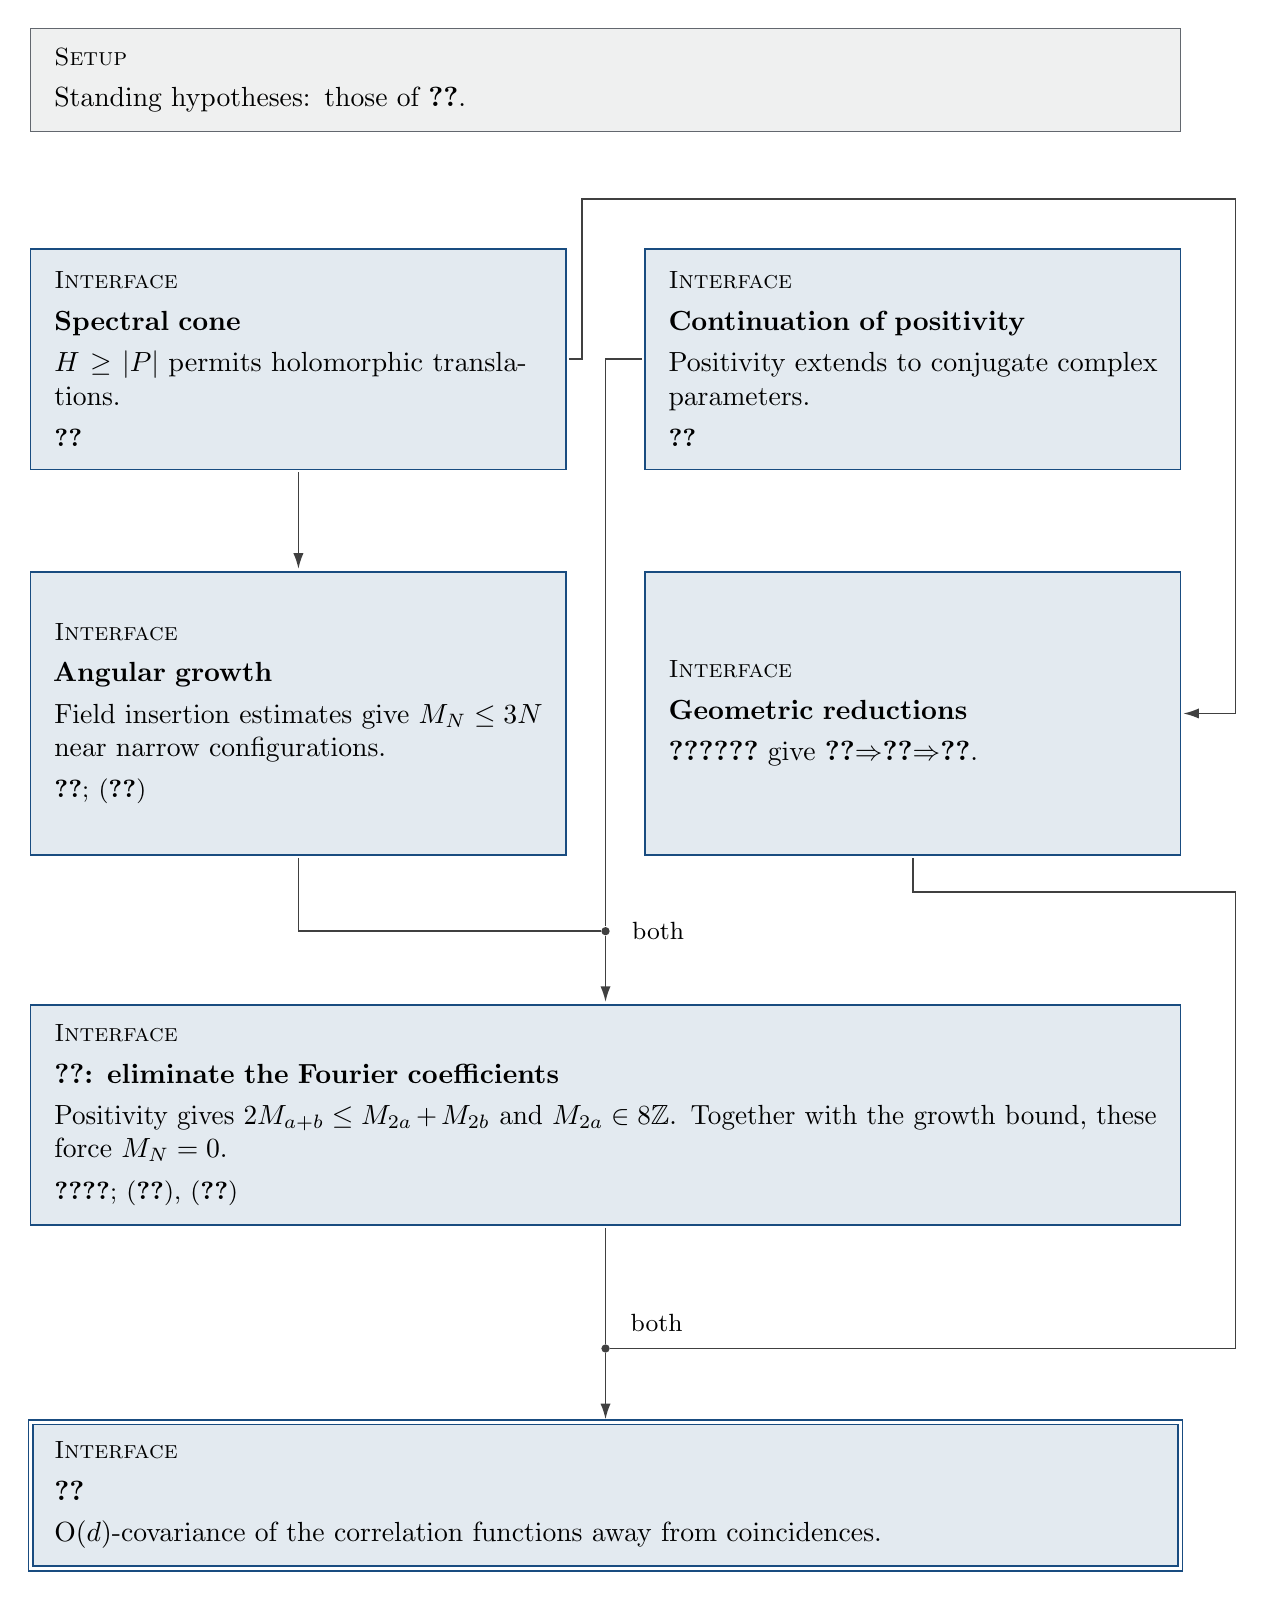
\begin{tikzpicture}[proof map]
\node[flow setup,text width=140mm,anchor=north] (standing) at (0,0) {
  \FlowRole{Setup}
  Standing hypotheses: those of \Cref{thm:main}.};

\node[flow interface,text width=62mm,minimum height=28mm,anchor=north]
  (cone) at (-39mm,-28mm) {
  \FlowRole{Interface}
  \FlowHeading{Spectral cone}
  $H\geq|P|$ permits holomorphic translations.
  \FlowRef{\Cref{prop:cone}}};
\node[flow interface,text width=62mm,minimum height=28mm,anchor=north]
  (positivity) at (39mm,-28mm) {
  \FlowRole{Interface}
  \FlowHeading{Continuation of positivity}
  Positivity extends to conjugate complex parameters.
  \FlowRef{\Cref{lem:analytic-positivity}}};

\node[flow interface,text width=62mm,minimum height=36mm,anchor=north]
  (growth) at (-39mm,-69mm) {
  \FlowRole{Interface}
  \FlowHeading{Angular growth}
  Field insertion estimates give $M_N\leq3N$ near narrow configurations.
  \FlowRef{\Cref{prop:final-growth}; \eqref{eq:point-bound}}};
\node[flow interface,text width=62mm,minimum height=36mm,anchor=north]
  (geometry) at (39mm,-69mm) {
  \FlowRole{Interface}
  \FlowHeading{Geometric reductions}
  \Cref{lem:reduction,prop:narrowing,lem:small_angle} give
  \Cref{thm:weaker}$\Rightarrow$\Cref{thm:weak}$\Rightarrow$\Cref{thm:main}.};

\node[flow join] (fourierjoin) at (0,-115mm) {};
\node[flow label,right=2mm of fourierjoin] {both};
\node[flow interface,text width=140mm,anchor=north]
  (narrow) at (0,-124mm) {
  \FlowRole{Interface}
  \FlowHeading{\Cref{thm:weaker}: eliminate the Fourier coefficients}
  Positivity gives $2M_{a+b}\leq M_{2a}+M_{2b}$ and $M_{2a}\in8\bbZ$.
  Together with the growth bound, these force $M_N=0$.
  \FlowRef{\Cref{lem:testing,lem:integer};
    \eqref{eq:convexity}, \eqref{eq:8}}};

\node[flow join] (finaljoin) at (0,-168mm) {};
\node[flow label,above right=1mm and 2mm of finaljoin] {both};
\node[flow interface,flow target,text width=140mm,anchor=north]
  (main) at (0,-177mm) {
  \FlowRole{Interface}
  \FlowHeading{\Cref{thm:main}}
  $\operatorname{O}(d)$-covariance of the correlation functions
  away from coincidences.};

\draw[flow dependency] (cone.south) -- (growth.north);
% Route above positivity, then along the outside; no crossing in the gutter.
\draw[flow dependency] (cone.east) -- (-3mm,0 |- cone.east)
  -- (-3mm,-22mm) -- (80mm,-22mm)
  -- (80mm,0 |- geometry.east) -- (geometry.east);
\draw[draw=black!75,line width=.65pt]
  (positivity.west) -- (0,0 |- positivity.west) -- (fourierjoin);
\draw[draw=black!75,line width=.65pt]
  (growth.south) |- (fourierjoin);
\draw[flow dependency] (fourierjoin) -- (narrow.north);
\draw[draw=black!75,line width=.65pt] (narrow.south) -- (finaljoin);
\draw[draw=black!75,line width=.65pt]
  (geometry.south) -- (39mm,-110mm) -- (80mm,-110mm)
  -- (80mm,-168mm) -- (finaljoin);
\draw[flow dependency] (finaljoin) -- (main.north);
\end{tikzpicture}
\par\smallskip
\FlowLegend
\caption{Principal steps in the proof. Here $M_N$ is the largest absolute
angular Fourier frequency at order $N$ near narrow configurations.
Arrows record inputs used under the standing hypotheses; both branches
at each junction are required. The geometric reductions use analyticity
under translations of separated groups.}
\label{fig:proof-overview}
\end{figure}
\clearpage

\section{Reductions}


For each pair $j<k$, consider the subgroup $G\subset \operatorname{SO}(d)$ consisting of orthogonal transformations $R$ that mix the two coordinates $x_j,x_k$ among themselves and leave the other coordinates fixed.
Because $\operatorname{SO}(d)$ is generated by the union of such subgroups, in order to prove full rotation covariance it suffices to prove covariance for transformations lying in each individual $G$, that is
\begin{equation}
    S_N(\chi) = S_N(R^* \chi )
\end{equation}
for all $N\in \bbN$, $R\in G$, and $\chi\in \calS_N$. 
The hypotheses of the theorem are invariant under a permutation of the coordinates, so it suffices to consider the group
\begin{equation}
    G=\Bigg\{  R(\theta) =\begin{bmatrix} 
    r(\theta) & 0 \\
     0 & I_{d-2} 
    \end{bmatrix}  : \theta\in \bbR
    \Bigg\} \cong \operatorname{SO}(2),\qquad  r(\theta) = 
    \begin{bmatrix}
        \cos \theta & \sin \theta \\ 
        -\sin \theta & \cos \theta 
    \end{bmatrix}
\end{equation}
of orthogonal transformations of the $tx$-plane. 

For each $N$-tuple $\chi=(\chi_1,\dots,\chi_N)\in \calS_N$
and $\theta\in \bbR$, define 
\begin{equation}
    D_N[\chi](\theta) = 
    S_N (R(\theta)^* \chi) -S_N(\chi)
\end{equation}
to measure the failure of $S_N$ to be rotation-invariant. 
Because $S_N$ is a distribution, $D_N[\chi] \in C^\infty(\bbS^1_\theta)$.\footnote{The notation $D_N[X](\theta)$ below is distributional shorthand: to say that it vanishes near $X$ means that the distribution $D_N(\theta)$ annihilates every test supported in some neighborhood of $X$. No pointwise evaluation at $X$ is assumed.} Note that $D_N[\chi](0)=0$. We want to show that
\begin{equation}
    D_N[\chi](\theta)=0
\end{equation}
for all $\theta$. 

Let $\Delta_2\subset (\bbR^d)^N$ be the set of configurations $X$ of points $\bfx=(t,x,y)$ such that the $(t,x)\in \bbR^2$ are not all distinct. In other words, if we let $\Pi:\bbR^d\to \bbR^2$ denote projection onto the first two coordinates, then $X\in (\bbR^d)^N$ lies outside $\Delta_2$ if and only if all points $\bfx\in X$ have distinct projections $\Pi \bfx$. 
We prove:
\begin{theorem}\label{thm:weak}
    Let $\mu:\operatorname{Borel}(\calS')\to [0,1]$ denote a Borel probability measure on $\calS'$. Denote its characteristic function by $\Phi$. Suppose that $\mu$ satisfies the following three properties:
    \begin{enumerate}[label=(\roman*)]
        \item  There exists a constant $C>0$ such that 
    \begin{equation}
        \int_{\calS'} e^{F(\chi)} \dd \mu(F) \leq e^{C(\lVert\chi\rVert_{L^1}+\lVert\chi\rVert_{L^2}^2)}
    \end{equation}
    for every real $\chi\in\calS$. 
    \item  
    The measure is invariant under spacetime translations. That is, for any $T:\bbR^d\to \bbR^d$ of the form $T(\bfx)=\bfx+\bfa$ for $\bfa\in \bbR^d$, 
    \begin{equation}
        \Phi(T^* \chi) = \Phi(\chi). 
    \end{equation}
    \item
    The measure is reflection positive across the four hyperplanes 
    \begin{equation}
        \{t=0\},\quad \{x=0\},\quad \{t+x=0\},\quad \{t-x=0\}.
    \end{equation}
    \end{enumerate}
    Then $D_N(\theta)$ vanishes on $(\bbR^d)^N\backslash \Delta_2$ for each $\theta\in \bbR$. 
\end{theorem}


The conclusion of this theorem is not full Osterwalder--Schrader covariance, because it leaves open the possibility that $D_N$ be nonzero on $\Delta_2\supseteq \Delta $, rather than only $\Delta$. 
In order to deduce full Osterwalder--Schrader covariance (under the hypotheses of \Cref{thm:main}), an argument is required.
The argument exploits some real-analyticity of $D_N[X](\theta)$'s dependence on $X$ to deduce vanishing for $X\in \Delta_2\backslash \Delta$ from vanishing for $X\notin \Delta_2$. 
The analytic dependence we use is under translations of the points on
one side of a separating coordinate hyperplane, with the other points
fixed. This is stated for smeared moments in \Cref{lem:reduction}.
Analyticity along such translations propagates the vanishing of $D_N$
from a neighborhood of one configuration to neighborhoods of the
configurations reached by those translations, as follows.


To make this more precise, we define for each $\theta \in \bbR$ an equivalence relation $\sim_\theta$ on $(\bbR^d)^N\backslash \Delta$ as follows. Suppose $X_0,X_1 \in (\bbR^d)^N\backslash \Delta$ are two configurations for which there exists a one-parameter group of translations $\bbR\ni s\mapsto T(s)$ of $(\bbR^d)^N$ with the following properties:
\begin{itemize}
    \item $T(1) X_0= X_1$
    \item for $t\in [0,1]$, $T(t)X_0$ stays inside of $(\bbR^d)^N\backslash \Delta$, 
    \item  for some open neighborhood $O\ni X_0$, if $\chi\in \calS_N$ satisfies $\operatorname{supp} \chi \subset O$, then the function 
    \begin{equation}
        s\mapsto D_N[T(-s)^* \chi](\theta) 
    \end{equation}
    is real-analytic on some neighborhood of $[0,1]$. 
\end{itemize}
Then we write $X_0\sim_\theta X_1$. This defines a reflexive symmetric relation, which we extend to an equivalence relation by taking the transitive closure. Then, if $X_0\sim_\theta X_1$ and $D_N[X](\theta)$ vanishes near $X=X_0$, it also vanishes near $X=X_1$. 


 
Given a configuration $X_0\in (\bbR^d)^N\backslash \Delta$, let
$H\subset\bbR^d$ denote an affine hyperplane parallel to the coordinate axes and containing none of the points $\bfx\in X_0$. Then, $H$ divides the points in $X_0$ into two groups. Let $\bfn$ denote a unit vector normal to $H$. Use that vector to designate one side of $H$ as the forward direction.
The following lemma states that $S_N(X)$ is real analytic at $X=X_0$ in any direction moving only the points in the group on the forward side of the hyperplane. More precisely, letting $H_0$ be the hyperplane parallel to $H$ and passing through the origin:
\begin{lemma}\label{lem:reduction} 
Fix $X_0$ as above. 
For $\delta\bfx\in\bbR^d$, write
$\tau_{\delta\bfx}(\bfx)=\bfx+\delta\bfx$, and let $T_{\bullet}=T_\bullet[H]:(\bbR^d)^N\to (\bbR^d)^N$ denote the translation that acts via $\tau_{\bullet}$ on the $j$th $\bbR^d$ factor of $(\bbR^d)^N$ if the $j$th point $\in X_0$ lies on the designated side of $H$ (and leaves the other factors fixed.) Then, under the hypotheses of \Cref{thm:main},  there exists an open neighborhood $O\ni X_0$ such that if $\chi\in \calS_N$ is supported in $O$, then the function 
\begin{equation}
    (-\varepsilon,\infty) \times H_0\ni (s, \bfv) \mapsto S_N(T^*_{-s \bfn - \bfv } \chi)
\end{equation}
is real analytic on $(-\varepsilon, \infty)\times H_0$ for some $\varepsilon>0$. 
Under the hypotheses of only \Cref{thm:weak}, the same conclusion holds if the hyperplane is one of constant $t$ or $x$ and $\bfv$ stays in the $tx$-plane. 
\end{lemma}


The lemma is proved in \S\ref{subsec:cluster-analyticity}. Given the lemma above:
\begin{proof}[Proof of \Cref{thm:main} (from \Cref{thm:weak})]
Assume the hypotheses of \Cref{thm:main}. 
Then \Cref{thm:weak} applies, so $D_N[X](\theta)$ vanishes for $X\in (\bbR^d)^N\backslash \Delta_2$. 
Consider a configuration $X\in \Delta_2\backslash \Delta$.
We prove that there exists some $X_0 \in (\bbR^d)^N\backslash \Delta_2 $ such that 
\begin{equation}
    X\sim_\theta X_0 
\end{equation}
for all $\theta\in \bbR$. In light of the discussion above, this will complete the proof: the vanishing of $D_N$ near $X_0$ implies the vanishing near $X$.
The move is to separate two points with equal planar projection by a
hyperplane in a $y$ coordinate and translate one side in time. That
hyperplane is fixed by $R(\theta)$, so the two terms of $D_N$ can both
be varied analytically using the same separating hyperplane. 

    For each $\#=0,\dots,1+N(N-1)/2$, let $\Delta_2^\#$ denote the set of configurations $X\in (\bbR^d)^N$ such that either $X\in \Delta$ or there exists a set of at least $\#$ pairs of distinct $\bfx,\bfx'\in X$ such that $\Pi \bfx=\Pi \bfx'$. Then 
    \begin{equation}
        (\bbR^d)^{N}=\Delta_2^0\supseteq \Delta_2=\Delta_2^1\supseteq \cdots \supseteq   \Delta_2^{1+N(N-1)/2}=\Delta  .
    \end{equation}

    Given $X\in (\bbR^d)^N\backslash \Delta$,
    let $\#$ be the smallest nonnegative integer such that $X\in \Delta_2^\#\backslash \Delta_2^{\#+1}$. 
    If $\#=0$, then $X\in (\bbR^d)^N\backslash \Delta_2$ already.
    If instead $\#\geq 1$, let $\bfx,\bfx'\in X$ denote two points in the configuration whose first two coordinates agree:
    \begin{equation}
        \Pi \bfx = \Pi \bfx'. 
    \end{equation}
    Because $X\notin \Delta$, the points $\bfx,\bfx'$ are distinct, so they must be distinguished by one of the remaining cartesian coordinates $y_1,\dots,y_{d-2}$. 
    Now pick a hyperplane $H=\{y_\bullet = a\}$ not containing any of the points in $X$ and separating $\bfx,\bfx'$.  

    
    Above, we defined $T_\bullet$. Redefine this with the coordinate $y_\bullet$ in place of $t$, using the hyperplane $H$ to define the two groups of points. Thus, for each $\delta t,\delta x\in \bbR$, we have a translation $T_{\delta t,\delta x}$ (that does nothing to the $y$ coordinates), 
    \begin{equation}
        T_{\delta t,\delta x}:(t,x,y)\mapsto (t+\delta t,x+\delta x,y).
    \end{equation}
    Now note that if $\delta t$ is in some small punctured interval $(-\varepsilon,\varepsilon)\backslash \{0\}$, then 
    \begin{equation}
        T_{\delta t,0} X  \in (\bbR^d)^N\backslash \Delta_2^\# 
    \end{equation}
    because it removes the coincidence between $\bfx,\bfx'$ by changing the time coordinate of one but not the other (and as long as $\varepsilon$ is sufficiently small, no more coincidences are created). We will show that 
    \begin{equation}
        X\sim_\theta T_{\delta t,0} X .
    \end{equation}
    If we have already proved the claim for smaller values of $\#$, then $T_{\delta t,0} X\sim_\theta X_0$ for some $X_0\in (\bbR^d)^N\backslash \Delta_2$, hence $X\sim_\theta X_0$. 

     In terms of $S_N$, 
    \begin{align}
    \begin{split} 
        D_N[T_{-\delta t,0}^* \chi ](\theta) &= S_N[R(\theta)^* T_{-\delta t,0}^* \chi] - S_N[T_{-\delta t,0}^* \chi] \\
        &= S_N[T_{-(\cos \theta )\delta t, -(\sin \theta)\delta t}^* R(\theta)^*  \chi] - S_N[T_{-\delta t,0}^* \chi].
        \end{split} 
    \end{align}
    Applying \Cref{lem:reduction} with $y_\bullet$ in place of $t$, we conclude that the right-hand side above depends real analytically on $\delta t$ near $\delta t=0$, as long as $\chi$ is supported sufficiently close to the configuration $X$. Hence $X\sim_\theta T_{\delta t,0} X$.
\end{proof}

The remaining reduction makes the successive planar displacements lie
in a common cone of opening less than $\pi/2$. This is the geometry
that will permit continuation in every complex rotation angle.


Say that a configuration $X \in (\bbR^d)^N\backslash \Delta_2$ is \emph{narrow} if the points in $X$ can be listed in some order $\bfx_1,\dots,\bfx_N$ such that, for some unit vector $\bfn\in \bbR^2$, the differences $\Pi(\bfx_{1} - \bfx_{2}),\cdots , \Pi(\bfx_{N-1}-\bfx_N)\in \bbR^2$ all make angle $<\pi/4$ with $\bfn$. That is, 
\begin{equation}
    \frac{\bfn \cdot \Pi (\bfx_{n} - \bfx_{n+1} )}{|\Pi(\bfx_{n} - \bfx_{n+1})|} > \frac{1}{\sqrt{2}}
\end{equation}
for $n=1,\dots,N-1$. 

\begin{proposition}\label{prop:narrowing}
    Under the hypotheses of \Cref{thm:weak}, for any $X\in (\bbR^d)^N\backslash \Delta_2$, there exists a $\delta>0$ and narrow $X_0$ such that $X\sim_\theta X_0$ whenever $-\delta<\theta<\delta$. 
\end{proposition}
\begin{proof}
    First, we show that every $X\in (\bbR^d)^N\backslash \Delta_2$ is equivalent to a configuration in which all points have a distinct time coordinate. Indeed, proceed via induction on the number of pairs of points sharing a time coordinate. If two times agree, their $x$ coordinates differ. A line $x=a$ separating them and avoiding the configuration divides the points into two groups. Move one group by a sufficiently small amount in the time direction. At least one time coincidence disappears and no new one is created. The two groups remain strictly separated in the $x$ coordinate. By \Cref{lem:reduction}, the moment is analytic along this move. For $|\theta|$ small, the rotated groups remain strictly separated in the $x$ coordinate throughout the move, so the other term in $D_N$ is analytic as well. Thus this move is allowed in $\sim_\theta$.

    Now suppose that $X\in (\bbR^d)^N\backslash \Delta_2$ contains points with distinct time coordinates. Then by a series of $T_{\delta t,0}$ for different hyperplanes, we can stretch $X$ in the vertical direction until the result is a narrow configuration: cut between successive times and move the later group forward until each successive time difference exceeds the absolute difference of the corresponding $x$ coordinates. Every move preserves strict time ordering. Each path is compact, so the same is true after rotation through sufficiently small $|\theta|$. Apply \Cref{lem:reduction} to both terms of $D_N$ along each path, and take the smallest of the finitely many allowed angle bounds. This gives the claimed $\delta$. The same choices work for configurations in a sufficiently small neighborhood of $X$.
\end{proof}

We now state:
\begin{theorem}\label{thm:weaker}
    Under the hypotheses of \Cref{thm:weak}, $D_N[X](\theta)$ vanishes on the set of narrow configurations $X$.
\end{theorem}

Given the theorem above:
\begin{proof}[Proof of \Cref{thm:weak} from \Cref{thm:weaker}]
    Given the hypotheses of the theorem, \Cref{thm:weaker} says that $D_N[X](\theta)$ vanishes whenever $X$ is narrow. By \Cref{prop:narrowing}, we conclude that given any $X\in (\bbR^d)^N\backslash \Delta_2$, there exists an open neighborhood $O\ni X$ and an interval about $\theta=0$ such that $D_N[\chi](\theta)=0$ whenever $\chi\in C_{\mathrm{c}}^\infty(O)$. 

    \Cref{lem:small_angle} completes the proof.   
\end{proof}





Given $X\in (\bbR^d)^N$, let $\calO(X)\subset (\bbR^d)^N$ denote the set of configurations arising by applying to $X$ a common rotation $R(\theta)$ to each point in the configuration. That is, $\calO(X)$ is $X$'s orbit under the group of rotations of the $tx$-plane.
\begin{lemma}\label{lem:small_angle}
     In order to show that $D_N(\theta)$ vanishes near some configuration $X\in (\bbR^d)^N\backslash \Delta$ for each $\theta\in \bbR$, it suffices to show that for each $X'\in \calO(X)$ there exists an open neighborhood $O\ni X'$ with the following property:  there exists a $\delta=\delta(O)>0$ such that $D_N[\chi](\theta)=0$ whenever $-\delta<\theta<\delta$ and $\chi \in \calS_N$ is supported in $O$. 
\end{lemma}
\begin{proof}
    Suppose that the desired neighborhoods exist. Because $\calO(X)$ is compact, a finite collection of the given neighborhoods covers it. Shrink $O_0\ni X$ and take the minimum of their angle bounds so that every rotated copy of $O_0$ lies in one of them.\footnote{Apply compactness to the parameter circle: each angle has an interval on which the corresponding rotated neighborhood remains in one fixed open set. A finite subcover gives both a common shrinkage of $O_0$ and a positive minimum angle bound.} Then the choice 
    \begin{equation} 
    O(X') = R(-\phi) O_0
    \end{equation} 
    works for $X'=R(-\phi)X$, with a common angle bound $\delta>0$.
    Now fix $\chi\in \calS_N$ supported in $O_0$, and consider the set 
    \begin{equation}
        \{\theta\in \bbR: D_N[\chi](\theta)=0\}.
    \end{equation}
    This is closed (because $\theta\mapsto D_N[\chi](\theta)$ is continuous) and contains $\theta=0$. 
    To see that it is open, hence all of the real line, suppose that $\theta_0$ lies in this set and $\theta$ satisfies $|\theta-\theta_0|<\delta$. By definition, 
    \begin{equation}
        D_N[\chi](\theta) = D_N[R(\theta_0)^* \chi ](\theta-\theta_0) + D_N[\chi](\theta_0).
    \end{equation}
    Both terms on the right-hand side are zero.
\end{proof}



The rest of this paper is devoted to the proofs of \Cref{lem:reduction} and \Cref{thm:weaker}.


\section{Proof sketch}\label{sec:sketch}

We prove \Cref{thm:weaker} by excluding every nonconstant angular
Fourier coefficient near narrow configurations. Expanding in Fourier
series, write
\begin{equation}\label{eq:fourier_integral}
 D_N[\chi](\theta)=\sum_{\ell\in\bbZ}c_\ell^{(N)}[\chi]e^{i\ell\theta},
 \qquad c_\ell^{(N)}[\chi]=\frac1{2\pi}\int_0^{2\pi}
 D_N[\chi](\theta)e^{-i\ell\theta}\dd\theta.
\end{equation}
It suffices to show that $c_\ell^{(N)}=0$ for $\ell\neq0$: the
remaining constant is zero because $D_N[\chi](0)=0$.\footnote{We
suppress $N,\chi$ when possible. For real tests,
$c_{-\ell}[\chi]=\overline{c_\ell[\chi]}$.}

The first step bounds the possible frequencies. Reflection positivity
across $t=0$ constructs the Osterwalder--Schrader Hilbert space and
the time and spatial translation generators $H,P$. Comparing this
construction with the one for $t+x=0$ gives $H\geq|P|$. At a spectral
point $(\omega,p)$ this says $|p|\leq\omega$, so
\[
 |e^{-t\omega+ixp}|\leq
 e^{-\omega(\Re t-|\Im x|)}.
\]
Thus translations extend holomorphically to
$q(t,x):=\Re t-|\Im x|>0$. Write $z_j=(t_j,x_j)$ for the complex
planar variables. We represent moments by fields inserted between
these complex translations. The regularity bound controls the
insertions and, for fixed transverse profiles, bounds the kernel by
a constant times $\bigl(1+(\min_{j<N}q(z_{j+1}-z_j))^{-1}\bigr)^N$.
The transverse variables remain smeared, so the power is independent of $d$.
For a narrow configuration, a suitable quarter turn puts the rotated
successive differences in $q>0$ at each real angle. Imaginary rotation
preserves this domain and satisfies
$q(R(-i\beta)z)\geq e^{-|\beta|}q(z)$. The kernel bound therefore
contributes $e^{N|\beta|}$. For the tensor action at these complex
angles, we use the complexification $\calT_\bbC$. The weight assumption
gives
\begin{equation}\label{eq:tensor-growth}
 \|\rho(R(\theta+i\beta))v\|\leq e^{2|\beta|}\|v\|,
 \qquad v\in\calT_\bbC.
\end{equation}
For two-forms the exponent can be replaced by $|\beta|$.
The tensor weights thus contribute at most $e^{2N|\beta|}$.
Hence, for tests near narrow configurations,
\begin{equation}\label{eq:angular-growth-preview}
 |D_N[\chi](\theta+i\beta)|\leq C_\chi e^{3N|\beta|}.
\end{equation}
Shifting the Fourier integral to height $\beta$ gives
$|c_\ell[\chi]|\leq C_\chi e^{3N|\beta|+\ell\beta}$.
Choose the sign of $\beta$ opposite to $\ell$ and let
$|\beta|\to\infty$: every coefficient with $|\ell|>3N$ vanishes.
The quarter turn is already a symmetry, so only $\ell\in4\bbZ$
can occur.

At order $N$, let $M_N$ be the largest absolute value of a nonzero
frequency occurring near some narrow configuration, and set $M_N=0$
if there is none. Thus $M_0=0$ and $0\leq M_N\leq3N$.
To eliminate the remaining frequencies, we compare moments of orders
$a+b$, $2a$ and $2b$ by reflection positivity. A narrow configuration
can be rotated and split by the reflection plane into groups of any
prescribed sizes $a,b$. The mixed reflected tuple and the two tuples
defining its squared norms all remain narrow. Consequently the same
Fourier bounds apply to all three; \S\ref{subsec:narrow-testing}
gives the precise support conditions.

This comparison must hold at imaginary rotation angles, where the
Fourier frequencies become exponential growth rates. We therefore
continue the positive reflection form itself, using
\Cref{lem:analytic-positivity}. For products $A,B$ of $a,b$ fields
with tuples $\chi,\eta$ as above, the resulting positive form is
\[
 \langle A,B\rangle_\beta
 =S_{a+b}(J\chi,\eta)+D_{a+b}[J\chi,\eta](i\beta),
 \qquad\beta\in\bbR,
\]
where $J\chi$ is the reflected, conjugated tuple. If the coefficient
at $-M_{a+b}$ is nonzero, the mixed pairing has a nonzero leading
term proportional to $e^{M_{a+b}\beta}$ as $\beta\to+\infty$.
Its two squared norms grow at most as $e^{M_{2a}\beta}$ and
$e^{M_{2b}\beta}$. Cauchy--Schwarz bounds the square of the mixed
pairing by their product; comparison of the exponents gives
\begin{equation}\label{eq:convexity-preview}
 2M_{a+b}\leq M_{2a}+M_{2b}.
\end{equation}
This is the convexity inequality used below.

There is a second restriction on the even orders. Suppose $M_{2a}>0$
and restrict the continued form to products of $a$ fields of the type
just described. Multiplying it by $e^{-M_{2a}\beta}$ and letting
$\beta\to+\infty$ gives a nonzero positive semidefinite form whose
entries are the leading coefficients. Some diagonal coefficient is
therefore strictly positive: otherwise Cauchy--Schwarz would
make every entry zero. Now rotate the law through $45^\circ$. This
permutes the four required reflection hyperplanes, so the rotated
law satisfies the same hypotheses and its corresponding diagonal
coefficient is nonnegative. But that coefficient is multiplied by
$e^{-iM_{2a}\pi/4}=(-1)^{M_{2a}/4}$. Its sign can be preserved only
if $M_{2a}\in8\bbZ$.

We therefore prove the three conditions
\[
 M_N\leq3N,\qquad 2M_{a+b}\leq M_{2a}+M_{2b},\qquad
 M_{2a}\in8\bbZ.
\]
Together with $M_0=0$ and nonnegativity, these force every $M_N$ to
vanish by \Cref{lem:integer}. This gives \Cref{thm:weaker}; the
geometric reductions above then give the main theorem.


\section{Consequences of reflection positivity (RP)}\label{sec:RP}

\subsection{The Osterwalder--Schrader Hilbert space}

The reflected quotient and translation semigroup follow the
Osterwalder--Schrader construction \cite[\S4.1, (4.3)--(4.9)]{OS}.
We use the ambient $L^2(\mu)$ bound in the contraction argument and
recall the details without assuming continuous rotation covariance.

Here we complexify the observable space to $L^2(\calS',\mu)_\bbC$.
Let $L^2_{+,\bbC}$ denote its closed subspace generated by observables
depending on fields in the forward half-space
$\{t>0\}$. In particular, it contains all products
\begin{equation}
 \operatorname{eval}_\chi(F)=F(\chi_1)\cdots F(\chi_N)
\end{equation}
with the tests supported there, and $\operatorname{eval}_\varnothing=1$.
We include the constant and allow complex coefficients in the algebra of such products.
These polynomials are dense in $L^2_{+,\bbC}$.\footnote{The regularity bound
allows the Taylor polynomials of $e^{iF(\chi)}$ to converge in $L^2$.
Field exponentials have dense span: a function orthogonal to them has
finite-dimensional conditional measures with zero Fourier transform,
hence zero conditional expectations. Evaluations generate the
sigma-algebra; see \S\ref{sec:well-definedness}.}

Write $\Theta_\circ(t,x,y)=(-t,x,y)$ and set
$J_\circ A=\overline{A(\Theta_\circ^*F)}$. Reflection invariance makes
$J_\circ$ an antiunitary involution on $L^2(\mu)_\bbC$. Define
\begin{equation}\label{eq:OS-form}
 \langle A,B\rangle_\circ=\bbE_\mu[(J_\circ A)B].
\end{equation}
The form is antilinear in its first argument. Reflection positivity is
equivalent to its being positive semidefinite on $L^2_{+,\bbC}$.
Indeed, on field exponentials its matrix is the transpose of the
characteristic-functional matrix in \Cref{it:RP}, and the transpose
of a positive Hermitian matrix is positive. The estimate
\begin{equation}\label{eq:class-contraction}
 |\langle A,B\rangle_\circ|\leq\|A\|_{L^2(\mu)}\|B\|_{L^2(\mu)}
\end{equation}
extends positivity to the closure. Conversely, applying positivity to
finite sums of exponentials gives the original condition.

Quotient by the null space and complete to obtain $\calH_{\circ,\bbC}$.
We conflate an observable with its class in this space, and put $\Omega=1$.
The quotient map is a contraction. Unmarked observable norms below are quotient
norms; ordinary probability-space norms carry an $L^p(\mu)$ subscript.

Let $T_{\delta t,\delta x}:(t,x,y)\mapsto
(t+\delta t,x+\delta x,y)$ denote a translation fixing $y$.
Its action on observables will mean $U(\delta t e_0+\delta x e_1)$.
For $s\geq0$, reflection and translation give
\begin{equation}
 \|U(se_0)A\|^2=\langle A,U(2se_0)A\rangle
 \leq\|A\|\,\|U(2se_0)A\|.
\end{equation}
Iterating and using $\|U(re_0)A\|\leq\|A\|_{L^2(\mu)}$ proves
contractivity and preservation of null vectors. The induced operators
are self-adjoint and strongly continuous. Translations parallel to
$t=0$ induce commuting strongly continuous unitary groups. Therefore
there are a nonnegative self-adjoint $H$ and a self-adjoint $P$ with
joint projection-valued measure $\Pi$ such that
\begin{equation}\label{eq:spectral-translations}
 V(\delta t,\delta x)=e^{-\delta tH+i\delta xP}
 =\int_{\bbR^2}e^{-\omega\delta t+ip\delta x}\dd\Pi(\omega,p),
 \qquad\delta t\geq0.
\end{equation}
They implement the translations of classes. Strong continuity follows
first on field exponentials from continuity of their tests and the
field moment bound, and then by density. The vacuum is fixed by every
translation. The same construction applies with any of the assumed
reflection hyperplanes as time zero.


\subsection{Spectral inequality}
Write $\Theta_\Delta(t,x,y)=(-x,-t,y)$ and $J_\Delta$ for its
antilinear reflection. Now consider the Hamiltonian $H$ and the
$x$-momentum generator $P$, constructed in the previous subsection
on the Osterwalder--Schrader Hilbert space.
\begin{proposition}\label{prop:cone}
    $H\geq |P|$
\end{proposition}
\begin{proof}
    Let $A\in L^2_{+,\bbC}$ denote a real polynomial in compactly supported field variables and $T=U(\delta t e_0+\delta x e_1)$ a translation with $\delta t>0$. Consider the quantity 
    \begin{equation}
        \bbE_\mu [(J_\circ A) T A]=\langle A,TA\rangle_{\calH_{\circ,\bbC}}.
    \end{equation}
    Letting $\rho = \langle A,  \Pi(-) A \rangle_{\calH_{\circ,\bbC}} :\operatorname{Borel}(\bbR^2)\to [0,\infty)$ denote the spectral measure associated to $A$, the right-hand side above is 
    \begin{equation}
        \langle A,T A \rangle_{\calH_{\circ,\bbC}} =  \int_{\bbR^2} e^{-\omega \delta t + i p \delta x} \dd \rho(\omega, p).
    \end{equation}
    Our goal is to show that $\rho$ is supported in the region $\{\omega\geq |p|\}$. Because the support of the spectral measure does not change upon translating $A$ forward in time, it suffices to replace $A$ by a 
    forward translate by a fixed $b>0$. Since our tests are compactly supported, by choosing $b$ large enough we may arrange that $A$ is supported in $\{t>|x|\}$. 

    Then $A$ and $J_\Delta J_\circ A$ are both tests in the  second Osterwalder--Schrader Hilbert space $\calH_{\Delta,\bbC}$. Thus, if $T$ maps the half space $\{t+x>0\}$ to itself, then
    \begin{equation}
        \bbE_\mu[(J_\circ A)T A ] =\bbE_\mu[J_\Delta (J_\Delta J_\circ A)T A ] = \langle J_\Delta J_\circ A,TA \rangle_{\calH_{\Delta,\bbC}}
    \end{equation}
    may be interpreted as an inner product in $\calH_{\Delta,\bbC}$. 
    The condition that $T_{\delta t,\delta x}$ map $\{t+x>0\}$ to itself says that $\delta t+\delta x\geq0$. Put $v=t+x$ and $u=t-x$.
    In $\calH_{\Delta,\bbC}$, the Hamiltonian $H_\Delta$ is the generator of translations in $v$, and $P_\Delta$ is the generator of translations in $u$. Hence 
    \begin{equation}
        T = \int_{\bbR^2} e^{- \omega (\delta t+\delta x) + i p (\delta t-\delta x)} \dd \Pi_\Delta(\omega,p) = \int_{\bbR^2} e^{ (ip-\omega) \delta t - (ip+\omega) \delta x} \dd \Pi_\Delta(\omega ,p) 
    \end{equation}
    where $\Pi_\Delta:\operatorname{Borel}(\bbR^2)\to \calB(\calH_{\Delta,\bbC})$ is the spectral measure for the pair $(H_\Delta,P_\Delta)$. So, letting $\rho_\Delta = \langle J_\Delta J_\circ A, \Pi_\Delta A \rangle_{\calH_{\Delta,\bbC}}$
    (this is a complex measure), we have 
    \begin{equation}
        \langle J_\Delta J_\circ A,TA \rangle_{\calH_{\Delta,\bbC}} = \int_{\bbR^2} e^{(ip-\omega) \delta t - (ip+\omega) \delta x} \dd \rho_\Delta(\omega,p)  .
    \end{equation}

    In summary, 
    \begin{equation}
        \int_{\bbR^2} e^{-\omega \delta t + i p \delta x} \dd \rho(\omega, p) = \bbE_\mu[(J_\circ A)T A ]=  \int_{\bbR^2} e^{(ip-\omega) \delta t - (ip+\omega) \delta x} \dd \rho_\Delta(\omega,p),
    \end{equation}
    This holds for all $\delta t>0$ and $\delta x>-\delta t$. 
    For the argument below, it is somewhat simpler to work with 
    \begin{equation}
        \delta v=\delta t +\delta x,\quad \delta u=\delta t-\delta x.
    \end{equation}
    Then, the identity above reads
    \begin{equation}
        \int_{\bbR^2} e^{\frac{1}{2}(ip-\omega)\delta v - \frac{1}{2} (\omega+ip)\delta u } \dd \rho(\omega, p) = \int_{\bbR^2} e^{-\omega \delta v +i p \delta u} \dd \rho_\Delta(\omega,p).
    \end{equation}
    In order to extract information about the measures $\rho,\rho_\Delta$,
    we integrate both sides of this equality against a function of the
    form $h(\delta v)\overline{h(\delta u)}$ for
    $h\in L^1((0,\infty))_\bbC$. Recall that 
    \begin{equation}
        \calL h(z) = \int_0^\infty e^{-zs} h(s) \dd s 
    \end{equation}
    denotes the Laplace transform of $h$. We now compute 
    \begin{align}
        \int_0^\infty \int_0^\infty h(\delta v) \overline{h(\delta u)} \int_{\bbR^2} e^{\frac{1}{2}(ip-\omega)\delta v - \frac{1}{2} (\omega+ip)\delta u } \dd \rho(\omega, p)  \dd \delta u \dd \delta v &= \int_{\bbR^2} \Big|\calL h\Big(\frac{\omega-ip}{2}\Big)\Big|^2  \dd \rho(\omega,p) \\ 
        \int_0^\infty \int_0^\infty  h(\delta v) \overline{h (\delta u)}\int_{\bbR^2} e^{-\omega \delta v +i p \delta u} \dd \rho_\Delta(\omega,p) \dd \delta u \dd \delta v &= \int_{\bbR^2} \calL h(\omega)\overline{\calL h(ip)} \dd \rho_\Delta(\omega,p) .
    \end{align}
    Thus, 
    \begin{align}\begin{split} 
        0 \leq \int_{\bbR^2} \Big|\calL h\Big(\frac{\omega-ip}{2}\Big)\Big|^2  \dd \rho(\omega,p) &= \int_{\bbR^2} \calL h(\omega)\overline{\calL h(ip)} \dd \rho_\Delta(\omega,p) \\
        &\leq \lVert \rho_\Delta \rVert \sup_{\omega\geq 0} |\calL h(\omega) |  \sup_{p\in \bbR} |\calL h(ip)|.
        \end{split} 
    \end{align}
    By Cauchy--Schwarz, $\lVert \rho_\Delta \rVert \leq \lVert J_\Delta J_\circ A\rVert_{\calH_{\Delta,\bbC}}\lVert A \rVert_{\calH_{\Delta,\bbC}}<\infty$. 

    Now the game is to find $h$ such that $\calL h$ is not too large on
    $\bbR^+\cup i\bbR$ but $\calL h$ is large at $(\omega-ip)/2$
    whenever $|p|>\omega$. Take $h(s)=s^{i\digamma}e^{-\varepsilon s}$,
    where $\varepsilon>0$ and $\digamma\in\bbR$ are parameters. This satisfies
    \begin{equation}
        \calL h(z)=\int_0^\infty s^{i\digamma}e^{-s(z+\varepsilon)}\dd s
        =C\Big(1+\frac z\varepsilon\Big)^{-1-i\digamma}
    \end{equation}
    for some numerical constant $C=C(\varepsilon,\digamma)\in\bbC^\times$.
    Thus,
    \begin{equation}
        |\calL h(z)|=|C|\cdot\Big|1+\frac z\varepsilon\Big|^{-1}
        e^{\digamma\operatorname{arg}(\varepsilon+z)}.
    \end{equation}
    Dividing out $|C|^2$, the inequality above reads
    \begin{equation}
        \int_{\bbR^2}\Big|1+\frac{\omega-ip}{2\varepsilon}\Big|^{-2}
        e^{2\digamma\operatorname{arg}(\varepsilon+z)}\dd\rho(\omega,p)
        \leq\lVert\rho_\Delta\rVert e^{\pi|\digamma|/2}
    \end{equation}
    for $z=(\omega-ip)/2$. The right-hand side is
    $O(e^{\pi|\digamma|/2})$ as $|\digamma|\to\infty$.
    But if $(\omega,p)\in\operatorname{supp}\rho$ and
    $|\operatorname{arg}(\varepsilon+z)|>\pi/4$, then for some $\eta>0$
    the left-hand side is $\Omega(e^{(\pi/2+\eta)|\digamma|})$
    as $\digamma\to+\infty$ or $\digamma\to-\infty$.\footnote{Choose a
    neighborhood of the point on which the argument is everywhere
    greater than $\pi/4+\eta/2$ or everywhere less than
    $-\pi/4-\eta/2$. Its $\rho$-measure is positive, as is its measure
    with the strictly positive weight $|1+z/\varepsilon|^{-2}$.
    Restricting the integral to this neighborhood gives the stated
    lower bound for the corresponding sign of $\digamma$.}
    These are only compatible if $|\operatorname{arg}(\varepsilon+z)|\leq\pi/4$,
    which means $\omega+2\varepsilon\geq|p|$.
    Taking $\varepsilon\to0$, we conclude $\omega\geq|p|$.\footnote{The
    preliminary forward translation multiplies the spectral measure by
    $e^{-2b\omega}>0$, so its support is unchanged. Polynomial classes
    with compact positive-time supports have dense complex span; hence
    the spectral projection of $\{\omega<|p|\}$ vanishes on
    $\calH_{\circ,\bbC}$.}
\end{proof}


\section{Extending reflection positivity}\label{sec:extend-RP}
\enlargethispage{2pt}

Reflection positivity is preserved under certain sorts of holomorphic
deformations of the reflection form. The lemma below is a
one-variable form of Glaser's positive-kernel continuation principle
\cite[Theorem~A]{Glaser}; we give the proof using derivative Gram
matrices and his Taylor-expansion argument
\cite[\S3, p.~14]{Glaser1969}.
\begin{lemma}\label{lem:analytic-positivity}
Let $\calX$ denote a vector space, let $j:\calX_\bbC\to L^2_{+,\bbC}$
be a map on its complexification, and let $O=O^*\subset\bbC$ denote a connected
open domain in the complex plane containing the origin. Say we have
chosen, for each pair of complex numbers $\xi,\zeta\in O$, a
sesquilinear form $\langle-,-\rangle_{\zeta,\xi}:\calX_\bbC^2\to\bbC$
such that
\begin{itemize}
\item for each $A,B\in\calX_\bbC$, the function
$(\zeta,\xi)\mapsto\langle A,B\rangle_{\zeta,\xi}$ is jointly
holomorphic on $O^2$;
\item for each $X\in\calX_\bbC$ there exists a $\delta>0$ and smooth
curve $[0,\delta)\ni s\mapsto X(s)\in L^2_{+,\bbC}$ such that $X(0)=j(X)$
and
\begin{equation}
 \langle A,B\rangle_{r,s}=\langle A(r),B(s)\rangle_\circ
\end{equation}
for all $r,s>0$ small enough.
\end{itemize}
Then, for each $z\in O$, the form
$\langle-,-\rangle_{z,\bar z}$ is positive semidefinite:
\begin{equation}
 \langle A,A\rangle_{z,\bar z}\geq0
\end{equation}
for all $A\in\calX_\bbC$.
\end{lemma}
Here $O^*=\{\bar z:z\in O\}$, and the forms are antilinear in their
first entry, consistently with \eqref{eq:OS-form}.

\begin{proof}[Proof idea]
Fix $A\in\calX_\bbC$.
To warm up, we show that $\langle A,A\rangle_{z,\bar z}\geq0$
for $z$ near the origin. Via analyticity, we may Taylor expand
\begin{equation}
 \langle A,A\rangle_{\zeta,\xi}
 =\sum_{a=0}^\infty\sum_{b=0}^\infty
 \frac{\zeta^a\xi^b}{a!b!}
 \partial_r^a\partial_s^b\langle A,A\rangle_{r,s}
 \Big|_{r=s=0}
\end{equation}
for $\zeta,\xi$ near $0$. The series on the right-hand side is
absolutely convergent. Now plug in $\zeta=z$ and $\xi=\bar z$:
\begin{equation}
\begin{split}
 \langle A,A\rangle_{z,\bar z}
 &=\sum_{a=0}^\infty\sum_{b=0}^\infty
 \frac{z^a\bar z^b}{a!b!}
 \partial_r^a\partial_s^b\langle A,A\rangle_{r,s}
 \Big|_{r=s=0}\\
 &=\lim_{N\to\infty}\sum_{a,b=0}^N
 \frac{z^a\bar z^b}{a!b!}
 \partial_r^a\partial_s^b\langle A,A\rangle_{r,s}
 \Big|_{r=s=0}.
\end{split}
\end{equation}
We can write the quantity under the limit as
\begin{equation}
 \sum_{a,b=0}^N\frac{z^a\bar z^b}{a!b!}
 \partial_\zeta^a\partial_\xi^b
 \langle A,A\rangle_{\zeta,\xi}\Big|_{\zeta=\xi=0}
 =v^\dagger M[N](0)v
\end{equation}
for $v=(v_0,\dots,v_N)\in\bbC^{N+1}$ the vector whose $j$th
component is $v_j=\bar z^j/j!$ and $M[N](z)$ the generally complex
matrix
\begin{equation}
 M[N](z)=
 \begin{bmatrix}
 \langle A,A\rangle_{\zeta,\xi}&\cdots&
   \partial_\xi^N\langle A,A\rangle_{\zeta,\xi}\\
 \vdots&\ddots&\vdots\\
 \partial_\zeta^N\langle A,A\rangle_{\zeta,\xi}&\cdots&
   \partial_\zeta^N\partial_\xi^N\langle A,A\rangle_{\zeta,\xi}
 \end{bmatrix}\Bigg|_{\zeta=z,\xi=\bar z}.
\end{equation}
The $(a,b)$th entry of $M[N](z)$ is
\begin{equation}\label{eq:reflection-derivative-matrices}
 M[N]_{a,b}(z)=\partial_\zeta^a\partial_\xi^b
 \langle A,A\rangle_{\zeta,\xi}\Big|_{\zeta=z,\xi=\bar z},
 \qquad0\leq a,b\leq N.
\end{equation}
If we know that $M[N](0)$ is positive semidefinite, then
$\langle A,A\rangle_{z,\bar z}\geq0$ follows.
To see that $M[N](0)$ is positive semidefinite, write
\begin{align}
\begin{split}
 M[N]_{a,b}(0)
 &=\partial_r^a\partial_s^b\langle A,A\rangle_{r,s}
       \Big|_{r=s=0}\\
 &=\partial_r^a\partial_s^b\langle A(r),A(s)\rangle_\circ
       \Big|_{r=s=0}\\
 &=\langle\partial_r^a A(r),\partial_s^b A(s)\rangle_\circ
       \Big|_{r=s=0}
 =\langle A^{(a)}(0),A^{(b)}(0)\rangle_\circ.
\end{split}
\end{align}
Thus, for every $v\in\bbC^{N+1}$,
\begin{equation}
 v^\dagger M[N](0)v
 =\Big\langle\sum_{n=0}^Nv_nA^{(n)}(0),
              \sum_{n=0}^Nv_nA^{(n)}(0)\Big\rangle_\circ\geq0,
\end{equation}
since $\langle-,-\rangle_\circ$ is positive semidefinite, as
desired.\footnote{One-sided derivatives at zero suffice. Smoothness
of the curves and continuity of the reflection pairing justify
differentiation; the derivatives remain in the closed space $L^2_{+,\bbC}$.}
\end{proof}

\begin{proof}
Fix $A$, and consider the subset $\Omega\subset O$ consisting of
$z\in O$ such that, for each $N\geq0$, the complex matrix $M[N](z)$
defined above is positive semidefinite.
Our goal is to show that $\Omega=O$. Indeed, if $M[N](z)$ is
positive semidefinite, then
\begin{equation}
 \langle A,A\rangle_{z,\bar z}
 =\bfe^\dagger M[N](z)\bfe\geq0
\end{equation}
for $\bfe=(1,0,\dots,0)$.

Because the matrix $M[N](z)$ depends continuously on $z$, the set
$\Omega$ is closed in $O$.
The sketch above contains the full proof that $0\in\Omega$, so
$\Omega$ is nonempty.
Next, we show that $\Omega$ is open, hence all of $O$ since $O$ is
connected. This is the general complex analytic fact in
\Cref{thm:analytic-open}, applied to the holomorphic function
$F(\zeta,\xi)=\langle A,A\rangle_{\zeta,\xi}$.
\end{proof}

The following is the one-variable derivative-positivity statement
in Glaser's argument \cite[\S3, p.~14]{Glaser1969}.\footnote{The same
Taylor re-expansion is given in \cite[Appendix~C, (145)--(146)]{BEM1998}.}
\begin{theorem}\label{thm:analytic-open}
Let $O\subset\bbC$ be open and invariant under complex conjugation,
and let $F:O^2\to\bbC$ be holomorphic. For $N\geq0$ define
\begin{equation}
 M_F[N](z)_{a,b}
 =\partial_\zeta^a\partial_\xi^bF(\zeta,\xi)
      \Big|_{\zeta=z,\xi=\bar z},\qquad0\leq a,b\leq N.
\end{equation}
Then the set
\begin{equation}
 \Omega_F=\{z\in O:M_F[N](z)\text{ is positive semidefinite
 for every }N\geq0\}
\end{equation}
is open in $O$.
\end{theorem}
\begin{proof}
Suppose $z_0\in\Omega_F$. Taylor expand
\begin{equation}
 \partial_\zeta^a\partial_\xi^bF(\zeta,\xi)
 =\sum_{\alpha,\beta\geq0}
 \frac{(\zeta-z_0)^\alpha(\xi-\bar z_0)^\beta}{\alpha!\beta!}
 \partial_\zeta^{a+\alpha}\partial_\xi^{b+\beta}F(z_0,\bar z_0)
\end{equation}
on a sufficiently small polydisc about $(z_0,\bar z_0)$.
This series is absolutely convergent. If $z$ is sufficiently close
to $z_0$, it follows that
\begin{equation}\label{eq:Taylor-matrices}
 M_F[N](z)=\lim_{L\to\infty}Z_LM_F[N+L](z_0)Z_L^\dagger,
\end{equation}
where $Z_L$ is the $(N+1)$-by-$(N+L+1)$ matrix with entries
\begin{equation}
 (Z_L)_{a,c}=\begin{cases}
 (z-z_0)^{c-a}/(c-a)!,&0\leq c-a\leq L,\\
 0,&\text{otherwise}.
 \end{cases}
\end{equation}
Indeed, the $(a,b)$ entry of the matrix under the limit is
\begin{equation}
 \sum_{\alpha,\beta=0}^L
 \frac{(z-z_0)^\alpha(\bar z-\bar z_0)^\beta}{\alpha!\beta!}
 \partial_\zeta^{a+\alpha}\partial_\xi^{b+\beta}F(z_0,\bar z_0),
\end{equation}
which converges to $M_F[N](z)_{a,b}$.
Each $Z_LM_F[N+L](z_0)Z_L^\dagger$ is the congruence of a positive
semidefinite matrix, hence positive semidefinite itself. Therefore,
for every $v\in\bbC^{N+1}$,
\begin{equation}
 v^\dagger M_F[N](z)v
 =\lim_{L\to\infty}(Z_L^\dagger v)^\dagger
       M_F[N+L](z_0)(Z_L^\dagger v)\geq0.
\end{equation}
The same polydisc works for every $N$, since all derivatives of $F$
are holomorphic there. Thus every $M_F[N](z)$ is positive
semidefinite for $z$ in one common neighborhood of $z_0$.
Consequently $z\in\Omega_F$, and $\Omega_F$ is open.
\end{proof}


\section{The analytic continuation}\label{sec:analytic}

The bound $|P|\leq H$ lets positive-time damping compensate for the
growth of imaginary spatial translations. Their spectral multipliers
have modulus at most $e^{-\omega(\Re t-|\Im x|)}$, so the quantity
below determines the complex translation domain.

For $z=(t,x)\in\bbC^2$ let
\begin{equation}\label{eq:tube}
 q(z)=\Re t-|\Im x|,\qquad\calW=\{z:q(z)>0\}.
\end{equation}
By \Cref{prop:cone}, the translation operators extend to
\begin{equation}\label{eq:complex-translations}
 V(z)=\int e^{-t\omega+ixp}\dd\Pi(\omega,p).
\end{equation}
They are contractions on $q\geq0$, strongly continuous there and
operator-norm holomorphic on $\calW$. Indeed, on $q\geq\delta>0$ a
spectral derivative of total order $k$ is bounded by
$\omega^ke^{-\delta\omega}\leq k!\delta^{-k}$, since $|p|\leq\omega$.
The semigroup law still holds, and $V(z)\Omega=V(z)^*\Omega=\Omega$.

\subsection{Analyticity across a separating hyperplane}
\label{subsec:cluster-analyticity}

We prove \Cref{lem:reduction}. Translate its separating hyperplane
to time zero, using its coordinate normal as the time direction.
Choose $\delta>0$ and the supports sufficiently close to the given
configuration that the negative group lies in $t<-\delta$ and the
positive group in $t>\delta$. Let $A_-$ and
$A_+$ denote the products of fields on the negative and positive
sides. Put
\begin{equation}
 \psi_-=U(-\delta\bfn)J A_-,\qquad
 \psi_+=U(-\delta\bfn)A_+,
\end{equation}
where $J$ is reflection in this hyperplane. Both define classes in
the Osterwalder--Schrader Hilbert space, and reflection and translation give
\begin{equation}\label{eq:cluster-matrix-element}
 \bbE_\mu[A_-U(s\bfn+\bfv)A_+]
   =\langle\psi_-,V(2\delta+s,\bfv)\psi_+\rangle.
\end{equation}
The ordinary pullback in the lemma is
$T_{-s\bfn-\bfv}^*$, exactly the translation $U(s\bfn+\bfv)$ here.

For a coordinate normal, repeat the cone argument with each other
coordinate as the transverse direction. The joint spectral variables
then satisfy $|p_i|\leq\omega$ for every tangential coordinate.
Consequently the right side of \eqref{eq:cluster-matrix-element} is
holomorphic whenever
\begin{equation}
 2\delta+\Re s>\sum_i|\Im v_i|.
\end{equation}
This proves the claimed real analyticity for $s>-2\delta$ and all
real $\bfv$. Under the four planar hypotheses the same argument uses
only the other planar momentum, proving the last assertion of the
lemma. If one of the groups is empty the moment is constant by
translation invariance. This completes the proof of
\Cref{lem:reduction}.

\subsection{A field in a time slab}\label{subsec:slab}

We need to insert a field between translations with a bound in the
Osterwalder--Schrader quotient norm. The ordinary $L^2(\mu)$ moment
bound does not by itself give this operator estimate. We first bound
an exponential insertion by repeated reflection, then differentiate
in its source. Below $K$ depends only on the constant $C$ in
\eqref{eq:gaussian} and may increase between estimates.

Repeated reflection doubles the time slab, the $L^1$ norm and the
squared $L^2$ norm of the source at each step. Cauchy--Schwarz takes
the corresponding $2^{-r}$ power, leaving the exponential bound
independent of the number of reflections.\footnote{We adapt the dyadic
Cauchy--Schwarz iteration in Seiler--Simon
\cite[Theorem~4.3, (23)--(24), p.~490]{SeilerSimon}. Their proof of
Theorem~7.1, (31)--(33), pp.~502--503, duplicates reflected sources;
the proof of Theorem~8.2, pp.~509--510, combines reflections with
Cauchy estimates for moments. Those results concern specific models;
here the terminal bound is \eqref{eq:gaussian}.}
We now extend $F$ complex-linearly to
$(L^1\cap L^2)(\bbR^d;\calT)_\bbC$ and its moments complex-multilinearly. Let $h$ belong to this space,
supported in $0\leq t\leq l$, and let $A$ be a bounded positive-time
observable. We claim
\begin{equation}\label{eq:slab-source}
 \|e^{F(h)}U(le_0)A\|\leq e^{C(\|\Re h\|_1+\|\Re h\|_2^2)}\|A\|.
\end{equation}
To prove this, reflection followed by translation gives
\begin{equation}
 \|e^{F(h)}U(le_0)A\|^2
 =\big\langle A,e^{F(\tau_{le_0}(Jh+h))}U(2le_0)A\big\rangle,
\end{equation}
where on tests $Jh=\Theta_\circ^*\bar h$. Define
\begin{equation}
 h_0=h,\quad h_{r+1}=\tau_{2^rle_0}(Jh_r+h_r),\quad
 a_r=\|e^{F(h_r)}U(2^rle_0)A\|.
\end{equation}
The source $h_r$ is supported in $0\leq t\leq2^rl$. Since the adjacent
slab interiors are disjoint,
\[
 \|\Re h_r\|_1=2^r\|\Re h\|_1,\qquad
 \|\Re h_r\|_2^2=2^r\|\Re h\|_2^2.
\] Cauchy--Schwarz gives
\begin{equation}
 a_r^2\leq\|A\|a_{r+1},\qquad
 a_0\leq\|A\|^{1-2^{-r}}a_r^{2^{-r}}.
\end{equation}
On the other hand, the defining reflection form and
\eqref{eq:gaussian} give
\begin{equation}
 a_r^2\leq\|A\|_{L^\infty(\mu)}^2
       \exp\bigl(C2^{r+1}(\|\Re h\|_1+\|\Re h\|_2^2)\bigr).
\end{equation}
Taking the square root and then the $2^{-r}$ power leaves the exponent
$C(\|\Re h\|_1+\|\Re h\|_2^2)$, while $\|A\|_{L^\infty(\mu)}^{2^{-r}}$
tends to one. The surviving dependence on $A$ is $\|A\|$, giving
\eqref{eq:slab-source} as $r\to\infty$.
If $\|A\|=0$, the first Cauchy--Schwarz inequality already gives $a_0=0$.

For $\chi$ supported in $|t|\leq\delta$, define
\begin{equation}\label{eq:slab-insertion}
 B_\delta(\chi)A=F(\tau_{\delta e_0}\chi)U(2\delta e_0)A.
\end{equation}
Apply Cauchy's estimate to the entire Hilbert-valued map
$z\mapsto e^{zF(\tau_{\delta e_0}\chi)}U(2\delta e_0)A$ on
$|z|=(\|\chi\|_1+\|\chi\|_2)^{-1}$ for $\chi\neq0$. Its power
series converges first in ordinary $L^2(\mu)_\bbC$, by
\eqref{eq:gaussian}. Equation~\eqref{eq:slab-source}
therefore gives
\begin{equation}\label{eq:insertion-bound}
 \|B_\delta(\chi)\|\leq K(\|\chi\|_1+\|\chi\|_2).
\end{equation}
The estimate shows that the insertion vanishes on null vectors and
therefore defines a bounded operator on $\calH_{\circ,\bbC}$.\footnote{Truncating $A$ in $L^4(\mu)_\bbC$ extends
\eqref{eq:slab-insertion} to the products of fields used below.
The field $L^4$ bound and H\"older's inequality justify the passage
to the quotient.}
Reflection and translation give
\begin{align}
 B_\delta(\chi)^*&=B_\delta(J\chi),\label{eq:insertion-adjoint}\\
 V(r+t,x)B_\delta(\chi)V(r-t,-x)
   &=B_{\delta+r}(\tau_{(t,x,0)}\chi),\qquad r\geq|t|.
 \label{eq:insertion-translation}
\end{align}
For example, both sides of \eqref{eq:insertion-translation} applied to
$A$ equal
$F(\tau_{(\delta+r+t,x,0)}\chi)U(2(\delta+r)e_0)A$.
If $\chi$ is supported in $|t-c|\leq\delta_0$ and
$|c|+\delta_0\leq\delta$, the same identity gives
\begin{equation}\label{eq:insertion-localization}
 B_\delta(\chi)=e^{-(\delta+c-\delta_0)H}
 B_{\delta_0}(\tau_{-ce_0}\chi)e^{-(\delta-c-\delta_0)H}.
\end{equation}

\subsection{Localizing an insertion in the plane}\label{subsec:point}

Fix a transverse profile $f\in(L^1\cap L^2)(\bbR^{d-2};\calT_\bbC)$.
For $d=2$ this means $f\in\calT_\bbC$, with both norms equal to $|f|$.
For planar $z=(t,x)$ put
\begin{equation}
 j_\varepsilon(z)=(\pi\varepsilon^2)^{-1}1_{\{|z|<\varepsilon\}},
 \qquad
 A_{f,\varepsilon}(\xi,\eta)
 =V(\xi-\varepsilon e_0)B_\varepsilon(j_\varepsilon f)
     V(\eta-\varepsilon e_0).
\end{equation}
This is defined for $q(\xi),q(\eta)>\varepsilon$. The slab estimate
alone gives the bound $K(\|f\|_1+\varepsilon^{-1}\|f\|_2)$, which diverges as
$\varepsilon\downarrow0$. We use holomorphy to bound the norm in terms
of $q_0=\min(q(\xi),q(\eta))$ instead. We claim
\begin{equation}\label{eq:regularized-point-bound}
 \|A_{f,\varepsilon}(\xi,\eta)\|
       \leq K\left(\|f\|_1+\frac{\|f\|_2}{q_0-\varepsilon}\right).
\end{equation}

We average translates of the insertion against a planar $L^2$ test.
Convolution by $j_\varepsilon$ contracts both $L^1$ and $L^2$;
the holomorphic mean-value inequality then recovers the value at
the center. Put $r=(q_0-\varepsilon)/2$ and, for unit vectors $u,v$, consider
$h_\varepsilon(\zeta)=
\langle u,A_{f,\varepsilon}(\xi+\zeta,\eta-\zeta)v\rangle$.
It is holomorphic for $|\Re\zeta_t|<r$, $|\Im\zeta_x|<r$.
Write $\zeta=z+ib$, with $z,b\in\bbR^2$. For $|b_x|<r$ the outer
factors
\begin{equation}
 V(\xi-(r+\varepsilon)e_0+ib),\qquad
 V(\eta-(r+\varepsilon)e_0-ib)
\end{equation}
are contractions, independent of $z$. Between them,
\eqref{eq:insertion-translation} identifies the remaining operator as
$B_{r+\varepsilon}((\tau_zj_\varepsilon)f)$ for
$z\in(-r,r)^2$. Thus, for $\alpha\in L^2((-r,r)^2)_\bbC$,
\begin{equation}
\begin{split}
 \left|\int\alpha(z)h_\varepsilon(z+ib)\dd z\right|
 &\leq K\bigl(\|f\|_1\|\alpha*j_\varepsilon\|_1
              +\|f\|_2\|\alpha*j_\varepsilon\|_2\bigr)\\
 &\leq K(2r\|f\|_1+\|f\|_2)\|\alpha\|_2,
\end{split}
\end{equation}
where $\alpha$ is extended by zero and $\|\alpha\|_1\leq2r\|\alpha\|_2$.
By duality, the $L^2((-r,r)^2)_\bbC$ norm of
$z\mapsto h_\varepsilon(z+ib)$ is at most $K(2r\|f\|_1+\|f\|_2)$.
The mean-value inequality on a complex polydisc
of radius $r'<r$, followed by integration over the imaginary square,
gives
\begin{equation}
 |h_\varepsilon(0)|^2\leq(\pi r'^2)^{-2}(2r)^2K^2
                    (2r\|f\|_1+\|f\|_2)^2.
\end{equation}
Let $r'\uparrow r$ and take the supremum over $u,v$ to prove
\eqref{eq:regularized-point-bound}.

We next identify the limit as $\varepsilon\downarrow0$. Fix
$\delta=q_0/2$, take $0<\varepsilon<\delta/2$, and let $\alpha$ be
supported in $(-\delta/2,\delta/2)^2$. Translation covariance gives
\begin{equation}\label{eq:point-identification}
 \int\alpha(z)A_{f,\varepsilon}(\xi+z,\eta-z)\dd z
 =V(\xi-\delta e_0)B_\delta((\alpha*j_\varepsilon)f)
           V(\eta-\delta e_0).
\end{equation}
The right side converges in operator norm because
$\alpha*j_\varepsilon\to\alpha$ in $L^1\cap L^2$.
For fixed vectors $u,v$, apply Montel's theorem to
$\langle u,A_{f,\varepsilon}(\xi+\zeta,\eta-\zeta)v\rangle$.
These scalar functions are locally uniformly bounded by
\eqref{eq:regularized-point-bound}. The norm limit in
\eqref{eq:point-identification} fixes the integral of every
subsequential limit against every test on the real square. Thus any
two limits agree there, and holomorphic uniqueness makes them agree
throughout the polydisc. Every sequence $\varepsilon\downarrow0$
therefore has the same scalar limit at $\zeta=0$. The limits are
bounded sesquilinear forms in $u,v$, hence define a bounded operator
$A_f(\xi,\eta)$ satisfying
\begin{equation}\label{eq:point-bound}
 \|A_f(\xi,\eta)\|\leq
 K\left(\|f\|_1+\frac{\|f\|_2}{\min(q(\xi),q(\eta))}\right).
\end{equation}
It is complex-linear in $f$. This insertion is localized only in the
plane; its transverse variables remain smeared. As $q_0\downarrow0$,
the $L^1$ term stays bounded and the $L^2$ term grows like $q_0^{-1}$,
independently of the number of transverse variables.

The translation and adjoint identities pass to the weak limit:
\begin{align}
 V(\kappa)A_f(\xi,\eta)V(\kappa')
   &=A_f(\kappa+\xi,\eta+\kappa'),\label{eq:point-shift}\\
 A_f(\xi,\eta)^*&=A_{Jf}(-\Theta_\circ\bar\eta,
                                      -\Theta_\circ\bar\xi).
 \label{eq:point-adjoint}
\end{align}
Here $q(\kappa),q(\kappa')\geq0$, and $Jf=\rho(\Theta_\circ)\bar f$
acts only on indices. The shift identity also proves norm holomorphy:
near $(\xi_0,\eta_0)$, choose small $a>0$ and factor the operator as
\begin{equation}
 V(\xi-\xi_0+ae_0)A_f(\xi_0-ae_0,\eta_0-ae_0)
          V(\eta-\eta_0+ae_0).
\end{equation}
For compactly supported $\alpha\in L^2(\bbR^2)$ with $|t|<\delta$
on its support, we recover the smeared insertion as
\begin{equation}\label{eq:smeared-point}
 B_\delta(\alpha f)=\int\alpha(z)
               A_f(\delta e_0+z,\delta e_0-z)\dd z.
\end{equation}
The integral converges in operator norm by \eqref{eq:point-bound}.
To verify the identity, take $\varepsilon$ smaller than half the distance
of the support to $|t|=\delta$. Equation~\eqref{eq:insertion-translation}
gives the regularized identity
\begin{equation}
 \int\alpha(z)A_{f,\varepsilon}(\delta e_0+z,\delta e_0-z)\dd z
       =B_\delta((\alpha*j_\varepsilon)f).
\end{equation}
The right side converges in norm to $B_\delta(\alpha f)$.
On the left, the matrix elements converge under a uniform bound
on the compact support, giving \eqref{eq:smeared-point}.
The product below depends on its two middle arguments only through
their sum: if $a,b,a',b'\in\calW$ and $a+b=a'+b'$, then
\begin{equation}\label{eq:gap-splitting}
 A_f(\xi,a)A_g(b,\eta)=A_f(\xi,a')A_g(b',\eta).
\end{equation}
Subtract a sufficiently small $\delta e_0$ from $a,b,a',b'$
and apply \eqref{eq:point-shift}. Both sides equal
$A_f(\xi,\delta e_0)V(a+b-2\delta e_0)A_g(\delta e_0,\eta)$.

\subsection{The ordered moment kernels}\label{subsec:ordered}

Composing the bounded insertions with successive translation
arguments gives a holomorphic kernel for the original ordered
moments. To write it, first take tests of the form
\begin{equation}
 \chi_j(t,x,y)=\alpha_j(t,x)f_j(y),\qquad
 f_j\in(L^1\cap L^2)(\bbR^{d-2};\calT_\bbC).
\end{equation}
Finite sums of these products suffice by density in $L^1\cap L^2$.\footnote{The
approximation can be made with prescribed planar supports; the moment
bound and multilinearity give the passage to general tests.}
For $N\geq2$ and $Z=(z_1,\dots,z_N)$ with
$\Delta_j=z_{j+1}-z_j\in\calW$, define
\begin{equation}\label{eq:ordered-kernel}
\begin{split}
 S_N(Z;f)=\big\langle\Omega,
 A_{f_1}(\kappa,\Delta_1/2)
 \Big[\prod_{j=2}^{N-1}A_{f_j}(\Delta_{j-1}/2,\Delta_j/2)\Big]
 A_{f_N}(\Delta_{N-1}/2,\kappa)\Omega\big\rangle.
\end{split}
\end{equation}
The product is ordered by increasing $j$ and is the identity if $N=2$.
The choice of $\kappa\in\calW$ does not matter: the shift identity and
$V\Omega=V^*\Omega=\Omega$ let any two choices be enlarged to a common
positive-time value. Put $S_0=1$ and
$S_1(z;f)=\langle m,\int f(y)\dd y\rangle$, with $m$ as in
\S\ref{subsec:setup}; in $d=2$ this is $\langle m,f\rangle$.

These kernels are holomorphic in the points, invariant under common
translations, and complex multilinear in the profiles. Taking
$\kappa$ with a sufficiently large time component in
\eqref{eq:point-bound} proves
\begin{equation}\label{eq:kernel-estimate}
 |S_N(Z;f)|\leq K^N\prod_{j=1}^N
      \left(\|f_j\|_1+q_*^{-1}\|f_j\|_2\right),
 \qquad q_*:=\min_{j<N}q(z_{j+1}-z_j).
\end{equation}
For compact planar supports strictly ordered in time, they represent
the original moments:
\begin{equation}\label{eq:ordered-density}
 S_N(\alpha_1f_1,\dots,\alpha_Nf_N)
 =\int\prod_j\alpha_j(z_j)S_N(Z;f)\dd Z.
\end{equation}
To check the identity, enclose the supports in disjoint slabs
$(c_j-\delta_j,c_j+\delta_j)$, ordered in $j$, and translate all of
them into positive time. Equations~\eqref{eq:slab-insertion} and
\eqref{eq:insertion-localization} express the class of the product as
\begin{equation}\label{eq:ordered-product}
 e^{-(c_1-\delta_1)H}B_{\delta_1}(\tau_{-c_1e_0}\chi_1)
 \Big[\prod_{j=2}^N e^{-(c_j-\delta_j-c_{j-1}-\delta_{j-1})H}
 B_{\delta_j}(\tau_{-c_je_0}\chi_j)\Big]\Omega.
\end{equation}
Insert \eqref{eq:smeared-point}. The semigroup law combines adjacent
translation factors with total argument $z_{j+1}-z_j$;
\eqref{eq:gap-splitting} assigns half of this argument to each
neighboring insertion. Pairing with $\Omega$ gives
\eqref{eq:ordered-density}. The successive time differences have a
positive lower bound on the compact supports, so the integrands are
uniformly bounded there. No product of fields at coincident points is used.

\subsection{Joining the ordered domains}\label{subsec:joining}

Permuting the entries gives every time ordering. Quarter turns give
the corresponding orderings with either $t$ or $x$ as time. On a
quarter-turned domain, rotate the points to the original domain and
apply the inverse pullback to their profiles. The kernels agree on
overlaps: the intersection is convex, and with every point it contains
its real part. A nonempty intersection therefore contains a real open
set, where both kernels give the original moments by
\eqref{eq:ordered-density}. Testing against products of smooth
functions and then applying the holomorphic identity theorem gives
equality on the intersection.

We continue to denote the joined kernel by $S_N(Z;f)$. Its real domain
contains the configurations for which either all times or all $x$
coordinates are distinct. It is symmetric under simultaneous
permutations of points and profiles. With
$\varrho(\zeta)=\rho(R(\zeta))$ acting on the tensor indices,
quarter-turn symmetry reads
\begin{equation}\label{eq:kernel-quarter}
 S_N(R(-\pi/2)Z;\varrho(\pi/2)f)=S_N(Z;f).
\end{equation}
This is the discrete symmetry already deduced from reflection
positivity, not the continuous covariance being proved.


\section{The growth estimate near narrow configurations}\label{sec:growth}

To bound the angular Fourier frequencies near narrow configurations,
we must continue $D_N[\chi]$ to every complex angle and control its
growth as the imaginary part tends to either infinity. Small real
angles suffice for the later geometric reductions, but the Fourier
contour shift requires this full continuation.

We retain the hypotheses of \Cref{thm:weak}. The ordered kernels and
the insertion estimates have already been constructed in
\S\ref{sec:analytic}; in particular, \eqref{eq:kernel-estimate} gives
\[
 |S_N(Z;f)|\le K^N\prod_{j=1}^N
       (\|f_j\|_1+q_*^{-1}\|f_j\|_2),
 \qquad q_*:=\min_{j<N}q(z_{j+1}-z_j).
\]

Fix a narrow planar configuration. Choose an ordering, a unit vector
$n$, and $\alpha<\pi/4$ so that all successive displacements lie
within angle $\alpha$ of $n$. Choose small product neighborhoods with
compact closures so that the same ordering, direction $n$, and
angle $\alpha$ work throughout them. Consider real product tests
\[
 \chi_j(t,x,y)=\alpha_j(t,x)f_j(y)
\]
with planar supports in these neighborhoods. Narrowness is an open condition.

\begin{proposition}\label{prop:final-growth}
If the planar tensor rotation weights have absolute value at most two,
then for each tuple of tests just described, $D_N[\chi]$ has an entire,
$2\pi$-periodic continuation satisfying
\begin{equation}\label{eq:final-growth}
 |D_N[\chi](\theta+i\beta)|\le C_\chi e^{3N|\beta|}
 \qquad(\theta,\beta\in\bbR).
\end{equation}
Consequently $c_\ell[\chi]=0$ for $|\ell|>3N$.
\end{proposition}

\begin{proof}
\emph{First cover every real angle.}
Write $n=R(\phi)(1,0)$. For any real $\theta$, choose an integer $k$ with
$|\theta-\phi-k\pi/2|\le\pi/4$. Each vector
$R(-\theta+k\pi/2)(z_{j+1}-z_j)$ then makes angle less than
$\alpha+\pi/4<\pi/2$ with the positive $t$-axis.
Thus
\begin{equation}\label{eq:final-real-gap}
 q\bigl(R(-\theta+k\pi/2)(z_{j+1}-z_j)\bigr)
 \ge \cos(\alpha+\pi/4)|z_{j+1}-z_j|.
\end{equation}
The integer $k$ may depend on $\theta$, but this bound does not. On the compact
product support its right side has a common positive lower bound,
denoted by $\delta$.

\emph{Extend each formula to its full vertical strip.}
The identity
\[
 q(z)=\min\{\Re(z_t+iz_x),\Re(z_t-iz_x)\}
\]
and the rotation convention give
\[
 (R(-i\beta)z)_t+i(R(-i\beta)z)_x=e^{-\beta}(z_t+iz_x),
 \qquad
 (R(-i\beta)z)_t-i(R(-i\beta)z)_x=e^{\beta}(z_t-iz_x).
\]
Consequently
\begin{equation}\label{eq:final-imaginary-gap}
 q(R(-i\beta)z)\ge e^{-|\beta|}q(z)\qquad(q(z)>0).
\end{equation}
In particular, imaginary rotations preserve the ordered domain.

For each integer $k$, the strict real-angle condition is
\begin{equation}\label{eq:final-strips}
 |\Re\zeta-\phi-k\pi/2|<\pi/2-\alpha.
\end{equation}
On this vertical strip, define the continuation of $D_N[\chi]$ by
\begin{equation}\label{eq:final-chart}
 \int\prod_j\alpha_j(z_j)
 S_N\bigl(R(-\zeta+k\pi/2)Z;
              \varrho(\zeta-k\pi/2)f\bigr)\,dZ-S_N(\chi).
\end{equation}
Here $\varrho$ acts on the profiles' tensor indices only, as in
\eqref{eq:kernel-quarter}.
The scalar tests are always evaluated at real points. Each vector
$R(-\zeta+k\pi/2)(z_{j+1}-z_j)$ lies in $\calW$, by
\eqref{eq:final-imaginary-gap}. On each compact subset of the strip,
the quantities $q(R(-\zeta+k\pi/2)(z_{j+1}-z_j))$ have a common
positive lower bound on the product support. The kernel bounds
therefore justify the integral and its holomorphy.

For real $\zeta$, \eqref{eq:final-chart} equals $D_N[\chi](\zeta)$:
apply the known quarter-turn covariance to the moment, and then use the
ordered smearing identity and a change of variables. This uses no
covariance under an arbitrary real rotation.
The strips \eqref{eq:final-strips} cover $\bbC$ and overlap, since
their width $\pi-2\alpha$ exceeds their center spacing $\pi/2$.
Any overlap contains a real interval, where both formulas equal
$D_N[\chi]$. The one-variable identity theorem makes the
formulas agree on the entire overlap and define a single entire
function. Replacing $\zeta$ by $\zeta+2\pi$ and $k$ by $k+4$ leaves
\eqref{eq:final-chart} unchanged, proving periodicity.

\emph{Estimate the continuation.}
For $\zeta=\theta+i\beta$, choose $k$ as in
\eqref{eq:final-real-gap}. Combining \eqref{eq:final-real-gap} and
\eqref{eq:final-imaginary-gap} gives
\[
 q\bigl(R(-\theta-i\beta+k\pi/2)(z_{j+1}-z_j)\bigr)
 \ge \delta e^{-|\beta|}.
\]
Thus $q_*^{-1}\leq\delta^{-1}e^{|\beta|}$ for the rotated tuple in
\eqref{eq:kernel-estimate}.

This is where representation theory enters. In an invariant norm, the
complexified planar rotation splits into weight spaces with factors
$e^{im\theta}$. If $|m|\le2$, then
\begin{equation}\label{eq:final-tensor}
 \|\varrho(\theta+i\beta-k\pi/2)f_j\|_p
 \le e^{2|\beta|}\|f_j\|_p,\qquad p=1,2.
\end{equation}
Real rotations preserve both norms. Each factor in
\eqref{eq:kernel-estimate} is therefore bounded by
$e^{3|\beta|}(\|f_j\|_1+\delta^{-1}\|f_j\|_2)$, uniformly in $k$.
Consequently
\begin{equation}\label{eq:final-rotated-kernel}
 \left|S_N\bigl(R(-\theta-i\beta+k\pi/2)Z;
                      \varrho(\theta+i\beta-k\pi/2)f\bigr)\right|
 \le K^N\prod_j(\|f_j\|_1+\delta^{-1}\|f_j\|_2)\,e^{3N|\beta|}.
\end{equation}
Integrating against the fixed scalar tests in \eqref{eq:final-chart}
proves \eqref{eq:final-growth} with $C_\chi$ independent of
$\theta,\beta$.\footnote{For example, one may take
$C_\chi=K^N\prod_j[\|\alpha_j\|_1(\|f_j\|_1+\delta^{-1}\|f_j\|_2)]+|S_N(\chi)|$.}
For a finite sum of such test products of the same order, sum the
corresponding constants.

Finally, shift the contour in \eqref{eq:fourier_integral}. The
continuation is entire and $2\pi$-periodic, so Cauchy's theorem on
the rectangle between heights $0$ and $\beta$ gives
\begin{equation}\label{eq:final-contour}
 \begin{split}
 c_\ell[\chi]
 &=\frac1{2\pi}\int_0^{2\pi}
 D_N[\chi](\theta+i\beta)e^{-i\ell\theta}e^{\ell\beta}\,d\theta,\\
 |c_\ell[\chi]|&\le C_\chi e^{3N|\beta|+\ell\beta}.
 \end{split}
\end{equation}
Periodicity cancels the vertical sides. Send $\beta\to+\infty$ when
$\ell<-3N$ and $\beta\to-\infty$ when $\ell>3N$. This proves the cutoff.
For $N=0,1$ the discrepancy is zero by $S_0=1$ and the covariance
of $S_1$ established in \S\ref{subsec:setup}.
\end{proof}

Quarter-turn symmetry makes $\theta\mapsto D_N[\chi](\theta)$
$\pi/2$-periodic;
holomorphic uniqueness gives the same periodicity for its entire
continuation. Hence only $\ell\in4\bbZ$ can occur. Since
$D_N[\chi](0)=0$, the cutoff gives, on these narrow tests,
\begin{equation}\label{eq:finite-defect}
 D_N[\chi](\zeta)
 =\sum_{\substack{\ell\in4\bbZ\\0<|\ell|\le3N}}
     c_\ell[\chi](e^{i\ell\zeta}-1).
\end{equation}
These are the original Fourier coefficients from
\eqref{eq:fourier_integral}. The moment bound makes each coefficient
a bounded multilinear form on $L^1\cap L^2$ tests, so density of finite sums
of product tests extends
\eqref{eq:finite-defect} to all tests with the same small compact planar
supports. The later positivity comparisons eliminate the remaining
frequencies on narrow configurations. The reductions in \S2, using
\Cref{lem:reduction}, then give $D_N[\chi](\theta)=0$ outside $\Delta$.


\subsection{Testing on narrow configurations}\label{subsec:narrow-testing}

Cauchy--Schwarz compares the reflected tuples $(J\chi,\eta)$,
$(J\chi,\chi)$ and $(J\eta,\eta)$. All three must be narrow for the
frequency bounds just proved to apply. The support conditions below
ensure this simultaneously. Write
\begin{equation}
 \calC_+=\{(t,x)\in\bbR^2:t>|x|\}.
\end{equation}
We use real product tests $\chi_j=\alpha_jf_j$, with
$\alpha_j\in C_c^\infty(\bbR^2;\bbR)$ and real transverse
$L^1\cap L^2$ profiles. Call an ordered tuple \emph{admissible} if its
compact planar supports $K_j=\operatorname{supp}\alpha_j$ satisfy
\begin{equation}\label{eq:admissible-supports}
 K_j\subset\calC_+,\qquad K_{j+1}-K_j\subset\calC_+.
\end{equation}
The empty tuple is included. All inequalities are strict and hold
for every choice of points in the supports.

For two admissible tuples $\chi,\eta$ with planar supports $K_j,L_k$,
the reflected concatenation
$(J\chi,\eta)$ is narrow. Reverse the first block to order it from
negative to positive time. Its successive displacement vectors are
those of the original tuple acted on by $-\Theta_\circ$, which
preserves $\calC_+$. When both tuples are nonempty, the displacement
from the last reflected point to the first unreflected point satisfies
\begin{equation}\label{eq:narrow-crossing}
 z'_1-\Theta_\circ z_1=z'_1+(-\Theta_\circ z_1)\in\calC_+,
 \qquad z_1\in K_1,\quad z'_1\in L_1,
\end{equation}
since both summands lie in $\calC_+$. Thus every successive
displacement vector lies in $\calC_+$, including for squared norms and mixed pairings
of different admissible tuples. A finite subdivision of the compact
supports therefore makes \eqref{eq:finite-defect} available for
all these pairings.

\begin{lemma}\label{lem:testing}
If $\ell\neq0$ and $c_\ell^{(N)}$ is nonzero near a narrow
configuration, then for every $a+b=N$ there are admissible tuples
$\chi,\eta$ of lengths $a,b$ such that
$c_\ell^{(N)}[J\chi,\eta]\neq0$.
\end{lemma}
\begin{proof}
The identity
\begin{equation}
 D_N[R(\phi)^*\chi](\theta)
   =D_N[\chi](\theta+\phi)-D_N[\chi](\phi)
\end{equation}
gives, directly from the Fourier integral,
\begin{equation}\label{eq:coefficient-rotation}
 c_\ell[R(\phi)^*\chi]=e^{i\ell\phi}c_\ell[\chi],
 \qquad\ell\neq0.
\end{equation}
Common translations and permutations also preserve the coefficients.
Localize a nonzero coefficient at a narrow configuration. Apply a common
rotation and order the planar points $z_1,\ldots,z_N$ so that
$z_{j+1}-z_j\in\calC_+$.
These operations preserve nonvanishing. If both groups are nonempty,
choose the origin at the
midpoint of $z_a,z_{a+1}$. For $j\leq a$ the vector from $z_j$ to
the midpoint is one half of $z_{a+1}-z_a$ plus a sum of successive
displacement vectors in $\calC_+$; for $j>a$ the vector from the
midpoint to $z_j$ has the same property.
Consequently the first group lies in $-\calC_+$ and the second in
$\calC_+$. Reflect and reverse the first group. Both tuples now
satisfy \eqref{eq:admissible-supports} on sufficiently small product
neighborhoods, where real product tests with nonzero coefficient
can be chosen.\footnote{By the Schwartz kernel theorem, a distribution
is nonzero on some product of tests in every product neighborhood
of a point in its support. Approximation by finite sums of
$\alpha(t,x)f(y)$ in $L^1\cap L^2$, followed by multilinearity and the
moment bound, gives the required real product tests.}
If one group is empty, put the origin sufficiently far forward or
backward in time instead. This proves the claim.
\end{proof}

\subsection{The continued reflection pairing}\label{subsec:continued-pairing}

The Fourier growth comparison needs a positive form at imaginary
rotation angles. We obtain a jointly holomorphic form by rotating the
two groups independently; for small real parameters it is their
ordinary reflection pairing. \Cref{lem:analytic-positivity} then gives
positivity at conjugate parameters, where the two groups undergo a
common imaginary rotation. Let $A=\prod_{j=1}^aF(\chi_j)$ and
$B=\prod_{k=1}^bF(\eta_k)$ be monomials with admissible tuples.
In particular, their supports are strictly ordered in $t>0$;
the two positive tuples may overlap each other.
For real $r,s$ small enough, put
\begin{equation}
 A(r)=\prod_jF(R(r)^*\chi_j),\qquad
 B(s)=\prod_kF(R(s)^*\eta_k).
\end{equation}
These are smooth $L^2_{+,\bbC}$ curves by the moment estimates.
Let $\calX$ be the real formal span of such monomials. On its
complexification $\calX_\bbC$, extend the forms sesquilinearly,
conjugating the first coefficient.
It suffices to work with any fixed finite family.\footnote{Formal
monomials give the natural map $j:\calX_\bbC\to L^2_{+,\bbC}$;
no choice of representation of an $L^2$ observable is needed. All
positivity and Cauchy--Schwarz assertions use only finite families.}

Write $\chi_j=\alpha_jf_j$ and $\eta_k=\gamma_kg_k$. Define
$\langle A,B\rangle_{\zeta,\xi}$ by integrating the ordered kernel
with its first group of points and profiles
\begin{equation}\label{eq:independent-rotations}
 R(\zeta)\Theta_\circ Z,\quad\varrho(-\zeta)Jf,
 \qquad\text{and its second group}\qquad
 R(-\xi)Z',\quad\varrho(\xi)g,
\end{equation}
against $\prod_j\alpha_j\prod_k\gamma_k$. List the reflected first
group in reverse order. Here $Jf=\rho(\Theta_\circ)\bar f$, and
$\varrho$ is precisely the tensor pullback in
\eqref{eq:kernel-quarter}. The relation
$\varrho(-r)\rho(\Theta_\circ)=\rho(\Theta_\circ)\varrho(r)$
fixes the signs in the first group. For small real $r,s$ the density
identity gives
\begin{equation}
 \langle A,B\rangle_{r,s}=\langle A(r),B(s)\rangle_\circ.
\end{equation}

For the fixed finite family choose $\delta>0$ so that rotations
with $|r|<\delta$ keep every positive support and every successive
displacement within each tuple in $\calC_+$. The kernel integral is
jointly holomorphic for
\begin{equation}
 (\zeta,\xi)\in O^2,\qquad O=\{z:|\Re z|<\delta\}.
\end{equation}
Indeed, the reflected points lie in $-\calW$ and the positive points
in $\calW$. Independent imaginary rotations preserve these cones
and the successive displacements within each tuple. The displacement
from the last reflected point to the first unreflected point is a
sum of two elements of $\calW$. On compact subsets of $O^2$ the insertion bounds are
uniform on the supports, justifying integration. Thus every
hypothesis of \Cref{lem:analytic-positivity} is satisfied.

At $(\zeta,\xi)=(-i\beta,i\beta)$ the two groups in
\eqref{eq:independent-rotations} are the same imaginary rotation of
the original reflected configuration. Their profiles are
$\varrho(i\beta)Jf$ and $\varrho(i\beta)g$. For real angles near zero
the integral agrees with the rotated moment. Holomorphic uniqueness
in the vertical strip, together with \eqref{eq:finite-defect}, gives
\begin{equation}\label{eq:continued-form}
 \langle A,B\rangle_\beta
 :=\langle A,B\rangle_{-i\beta,i\beta}
 =S_{a+b}(J\chi,\eta)+D_{a+b}[J\chi,\eta](i\beta),
 \qquad\beta\in\bbR.
\end{equation}
Here $J\chi$ is the reflected, conjugated tuple. Its concatenation
with $\eta$ is narrow by \eqref{eq:narrow-crossing}, which is why
the finite Fourier expansion \eqref{eq:finite-defect} applies.
The form on the left is positive semidefinite. Empty tuples give
the vacuum and are included in this statement. Positivity applies
to the continued moment in \eqref{eq:continued-form}.

\section{Eliminating Fourier coefficients}\label{sec:eliminating}

The degree comparison and the use of parity below adapt the arguments
of Streater's Lemmas~2 and~3 \cite[pp.~113--114]{Streater}; see also
Osipov \cite[p.~115]{O}. We distinguish the comparison with the law
rotated through $\pi/4$, which supplies the divisibility needed here.

We now finish the proof of \Cref{thm:weaker}. Let $M_N$ be the largest
$|\ell|$ for which $c_\ell$ is nonzero near some narrow configuration,
and set it to zero if all nonzero frequencies vanish there. Then
\begin{equation}\label{eq:M-bound}
 M_0=0,\qquad M_N\in4\bbZ,\qquad0\leq M_N\leq3N.
\end{equation}
The conjugation identity exchanges positive and negative frequencies,
so whenever $M_N>0$ the coefficient at $-M_N$ is nonzero as well.
These coefficients are invariant under common translations and
permutations of the entries. Translation invariance follows from
$R(\theta)^*\tau_a=\tau_{R(-\theta)a}R(\theta)^*$ in both terms
of $D_N$.

\subsection{$2M_{a+b}\leq M_{2a}+M_{2b}$}

We apply the leading-degree argument of Streater
\cite[Lemma~2, pp.~113--114]{Streater} to the positive continued
reflection form \eqref{eq:continued-form}.

Fix nonnegative integers $a,b$. If $M_{a+b}=0$, there is nothing to
prove, so assume $M_{a+b}>0$. By \Cref{lem:testing}, there are
admissible tuples $\chi,\eta$ of lengths $a,b$ such that
\begin{equation}
 c_{-M_{a+b}}[J\chi,\eta]\neq0.
\end{equation}
Equation~\eqref{eq:continued-form} and the finite Fourier expansion
\eqref{eq:finite-defect}, applied to this narrow tuple, give
\begin{equation}\label{eq:leading-growth}
 \langle A,B\rangle_\beta
   =\bigl(c_{-M_{a+b}}[J\chi,\eta]+o(1)\bigr)
                  e^{M_{a+b}\beta}\qquad(\beta\to+\infty).
\end{equation}
Similarly,
$\langle A,A\rangle_\beta=O(e^{M_{2a}\beta})$ and
$\langle B,B\rangle_\beta=O(e^{M_{2b}\beta})$.
All three tuples are narrow by the admissibility conditions.
The form is positive semidefinite, so Cauchy--Schwarz gives
\begin{equation}\label{eq:ext_CS}
 |\langle A,B\rangle_\beta|^2
       \leq\langle A,A\rangle_\beta\langle B,B\rangle_\beta.
\end{equation}
Since the leading coefficient in \eqref{eq:leading-growth} is nonzero,
comparison of the exponents yields
\begin{equation}\label{eq:convexity}
 2M_{a+b}\leq M_{2a}+M_{2b}.
\end{equation}

\subsection{$M_{2a}\in8\bbZ$}

We use the leading-term positivity argument of Streater
\cite[\S6, especially the proof of Lemma~8]{Streater}, here for the
continued reflection form.
Suppose that $M=M_{2a}>0$. Multiplying the positive form
$\langle-,-\rangle_\beta$ on admissible degree-$a$ monomials by $e^{-M\beta}$
and letting $\beta\to+\infty$ gives a positive semidefinite form
\begin{equation}
 (A,B)\longmapsto c_{-M}[J\chi,\eta].
\end{equation}
The testing lemma supplies $A,B$ for which this form is nonzero.
If every diagonal value were zero, Cauchy--Schwarz would make every
entry zero. Thus some diagonal value is strictly positive:
\begin{equation}\label{eq:c_pos}
 c_{-M}[J\chi,\chi]>0.
\end{equation}
This is a sign assertion about the leading coefficient of
$\langle A,A\rangle_\beta$; mixed Fourier coefficients need not have a sign.

The remainder of the argument involves studying the effect of a
$45^\circ$ rotation $Q=R(\pi/4)$ on the measure $\mu$. Define
$\tilde\mu$ by
\begin{equation}
 \tilde\Phi(\chi)=\Phi(Q^*\chi),\qquad
 \tilde S_N(\chi)=S_N(Q^*\chi).
\end{equation}
Since $Q$ permutes the four reflection hyperplanes,
reflection invariance and positivity, the regularity estimate and
translation invariance are preserved. These are all the hypotheses
used in the chosen plane, so the same argument applies to
$\tilde\mu$, in its own Hilbert space.

Since planar rotations commute,
\begin{equation}
 \tilde D_N[\chi](\theta)
       =D_N[\chi](\theta+\pi/4)-D_N[\chi](\pi/4).
\end{equation}
Matching the nonzero Fourier coefficients gives
\begin{equation}\label{eq:tilt-coefficient}
 \tilde c_\ell[\chi]=e^{i\ell\pi/4}c_\ell[\chi]
                  =(-1)^{\ell/4}c_\ell[\chi],
 \qquad\ell\in4\bbZ\setminus\{0\}.
\end{equation}
Nonvanishing is unchanged, so $\tilde M_N=M_N$.
Now use the positivity of $\tilde c_{-M}$ and $c_{-M}$ on the tuple
in \eqref{eq:c_pos}:
\begin{equation}
 0\leq\tilde c_{-M}[J\chi,\chi]
     =(-1)^{M/4}\underbrace{c_{-M}[J\chi,\chi]}_{>0}.
\end{equation}
Thus $(-1)^{M/4}=1$, which means $M\in8\bbZ$.
The zero case is automatic, so
\begin{equation}\label{eq:8}
 M_{2a}\in8\bbZ\qquad(a\geq0).
\end{equation}

It remains to combine the inequality between moment orders, the
even-order divisibility and the linear bound. The inequality makes
the even-order increments nondecreasing; divisibility prevents a
positive increment from being small enough to respect the bound.
The following lemma gives the version needed here.\footnote{The proof
of Streater's Lemma~3 \cite[p.~114]{Streater} likewise combines his
convexity inequality with linear growth and parity. Its numerical
statement and conclusion differ from those below.}
\begin{lemma}\label{lem:integer}
Suppose $0=M_0,M_1,M_2,\dots$ are nonnegative integers satisfying
\begin{equation}
 M_n\leq3n,\qquad2M_{a+b}\leq M_{2a}+M_{2b},\qquad
 M_{2n}\in8\bbZ
\end{equation}
for all nonnegative integers $a,b,n$. Then $M_n=0$ for every $n$.
\end{lemma}
\begin{proof}
Note that $0\leq M_2\leq6$ and $M_2\in8\bbZ$, so $M_2=0$.
Define $\delta_n=M_{2n}-M_{2n-2}$. Applying convexity, the second inequality, with
$a=n-1$ and $b=n+1$ yields
\begin{equation}
 2M_{2n}\leq M_{2n-2}+M_{2n+2},
\end{equation}
hence $\delta_n\leq\delta_{n+1}$. The increments are nondecreasing
multiples of eight and $\delta_1=0$, so all are nonnegative. If
$\delta_r$ were positive, it would be at least eight, as would every
later increment. This implies
\begin{equation}
 M_{2j}\geq M_{2r-2}+8(j-r+1)\geq8(j-r+1),
\end{equation}
contradicting $M_{2j}\leq6j$ for large $j$. Therefore every increment
vanishes, and $M_{2n}=0$. Finally,
$0\leq2M_n\leq M_0+M_{2n}=0$ controls the remaining terms.
\end{proof}

\begin{remark*}
Convexity \eqref{eq:convexity} makes the even-order increments
nondecreasing, and $M_{2n}\in8\bbZ$ makes them multiples of eight.
Once one is positive, every later increment is at least eight,
contradicting $M_{2j}\leq6j$ for sufficiently large $j$.
\end{remark*}

\section{Conclusion}

\Cref{lem:integer} gives $M_N=0$ for every $N$, so
\eqref{eq:finite-defect} gives $D_N[\chi](\theta)=0$ near every narrow
configuration. This proves \Cref{thm:weaker}. The narrowing and small-angle
arguments give \Cref{thm:weak}; the proof of \Cref{thm:main} from
\Cref{thm:weak} in \S2 then gives covariance under rotations of the
$tx$-plane.
The same proof applies to every coordinate plane. These rotations
generate $\operatorname{SO}(d)$, and the coordinate reflections
already preserve the law, so the conclusion holds for all of
$\operatorname{O}(d)$.

For compactly supported tests with pairwise disjoint supports this
is precisely the distributional vanishing off $\Delta$ established
above. General Schwartz tuples with pairwise disjoint supports
follow by compact truncation, which preserves disjointness, and
\eqref{eq:moment_bd}. The theorem concerns these
off-diagonal moments; no removal of contact terms has been used.


\section{Sharpness of the conclusion and the weight restriction}
\label{sec:sharpness-examples}
\enlargethispage{2pt}

The hypotheses permit noncovariant contact terms. Moreover, the
representation restriction cannot be enlarged uniformly to include
planar weight three. Both limitations already occur in dimension two.\footnote{The two
examples in this section were supplied in the referee report.}

\subsection{Noncovariant contact terms}

Let $\calT=\operatorname{Sym}^2_0(\bbR^2)$, with orthonormal basis
\[
 e_1=\frac{dt^2-dx^2}{\sqrt2},\qquad
 e_2=\frac{dt\otimes dx+dx\otimes dt}{\sqrt2}.
\]
Take independent scalar white noises in these two components, with
variances $a,b>0$, where $a\ne b$. Their characteristic function is
\[
 \Phi(\chi)=e^{-Q(\chi)/2},\qquad
 Q(\chi)=\int_{\bbR^2}(a\chi_1^2+b\chi_2^2).
\]
The law is translation invariant and satisfies
$\bbE e^{F(\chi)}\leq e^{\max(a,b)\|\chi\|_2^2/2}$.

In this basis the coordinate reflections act by
$\operatorname{diag}(1,-1)$ and the diagonal reflections by
$\operatorname{diag}(-1,1)$. They preserve $Q$. If the tests lie on
one side of any required mirror, their reflected supports are disjoint
from the original supports. Hence
\[
 \Phi(\chi_j-\Theta^*\chi_k)
 =e^{-Q(\chi_j)/2}e^{-Q(\chi_k)/2},
\]
a rank-one positive semidefinite matrix. Thus all the required
reflection positivities hold.

The tensor pullback of $R(\theta)$ is $R(-2\theta)$. At
$\theta=\pi/4$ it exchanges $e_1,e_2$, up to sign. Taking
$\chi=f e_1$ shows that $Q(\chi)=a\|f\|_2^2$, whereas
$Q(R(\pi/4)^*\chi)=b\|f\|_2^2$. The law is therefore not rotation
invariant. Its covariance kernel is
$\operatorname{diag}(a,b)\delta(q-q')$.
Every nonempty moment on pairwise disjoint supports nevertheless
vanishes, since the centered Gaussian evaluations are independent.
The failure of covariance is entirely supported at coincidences.

\subsection{Failure at planar weight three}

Let $\phi$ be the massive scalar Gaussian free field on $\bbR^2$,
with covariance $(-\Delta+m^2)^{-1}$, $m>0$. This field is reflection
positive; see the scalar covariance calculation and its Fock-space
extension in \cite[pp.~119--120]{Uhl79}.

Let $\calT_3$ be the two-dimensional space of real harmonic cubics.
Choose an orthonormal basis $(e_1,e_2)$ proportional to
\[
 t^3-3tx^2,\qquad 3t^2x-x^3.
\]
For the clockwise rotations used here,
\[
 \rho_3(R(\theta))=R(-3\theta),\qquad
 \rho_3(\Theta_\circ)=\operatorname{diag}(-1,1).
\]
Thus the planar weights are $\pm3$. Put $S=\operatorname{diag}(1,-1)$
and define the $\calT_3$-valued field by
\[
 F=(\partial_t\phi,-\partial_x\phi),\qquad
 F(\chi)=\phi(L\chi),\qquad L\chi=-\operatorname{div}(S\chi).
\]
For every symmetry $g$ of the square,
\[
 S\rho_3(g)=g^{\mathsf T}S.
\]
Indeed, this holds for a quarter turn and for $\Theta_\circ$, which
generate the group; the pullback multiplication order preserves the
identity. Since $gS\rho_3(g)=S$, the chain rule gives
\[
 L(g^*\chi)=(L\chi)\circ g.
\]
The map $L$ preserves supports and commutes with translations.
Consequently scalar reflection positivity transfers to the
characteristic function of $F$ across all four required mirrors.
The law is translation invariant.

With unitary Fourier transform,
\[
 \bbE F(\chi)^2
 =\int_{\bbR^2}
 \frac{|p_t\widehat\chi_1-p_x\widehat\chi_2|^2}
 {|p|^2+m^2}\dd p
 \leq\|\chi\|_2^2.
\]
Thus $\bbE e^{F(\chi)}\leq e^{\|\chi\|_2^2/2}$ for every real
test, with the required uniform $L^2$ bound.

It remains to check that covariance fails away from coincidences.
Write $h(r)$ for the scalar covariance at positive separation. The
matrix-valued covariance kernel is
\[
 K(z)=-S(D^2h)(z)S.
\]
For two first-component insertions initially separated by $(r,0)$,
the pullback rotates the separation to $r n_\theta=R(-\theta)(r,0)$
and the profile to $v_\theta=\rho_3(R(\theta))e_1$. In particular,
\[
 n_\theta=(\cos\theta,\sin\theta),\qquad
 S v_\theta=(\cos3\theta,-\sin3\theta),\qquad
 (S v_\theta)\cdot n_\theta=\cos4\theta.
\]
The radial Hessian formula therefore yields
\[
 v_\theta^{\mathsf T}K(rn_\theta)v_\theta
 =-\frac12\left(h''(r)+\frac{h'(r)}r\right)
  -\frac12\left(h''(r)-\frac{h'(r)}r\right)\cos8\theta.
\]
Its difference from the value at $\theta=0$ is
\[
 \frac12\left(h''(r)-\frac{h'(r)}r\right)(1-\cos8\theta).
\]
The coefficient is strictly positive. Indeed,
\[
 h(r)=\int_0^\infty
       \frac{e^{-m^2s-r^2/(4s)}}{4\pi s}\dd s,
 \qquad
 h''(r)-\frac{h'(r)}r
 =\int_0^\infty\frac{r^2}{4s^2}
       \frac{e^{-m^2s-r^2/(4s)}}{4\pi s}\dd s>0.
\]
For $r>0$, exponential decay at both ends justifies differentiating
under the integral. At $\theta=\pi/8$ the difference is nonzero.
Since the kernel is smooth away from the origin, the difference
remains nonzero after integration against suitable smooth tests
with sufficiently small disjoint supports.

This example has $M_2=8$. Allowing weight three would replace the
angular bound by $M_N\leq4N$, which permits this value. Hence the
cutoff two is sharp for a theorem covering every representation in
the stated class: the next integer cutoff already fails in dimension
two.

\appendix

\section{Well-definedness of \texorpdfstring{$S_N$}{SN}}\label{sec:well-definedness}

Fr\"ohlich \cite[Lemma~3.2, pp.~276--277]{Frohlich} obtains factorial
moment bounds from a uniform strip bound on the generating functional
by Cauchy's formula. For the present regularity bound, a tail estimate
gives the order dependence used in \eqref{eq:moment_bd}.

For real $\chi\neq0$, apply \eqref{eq:gaussian} to $u\chi$, $u\in\bbR$.
The exponential Markov inequality, optimized over positive and
negative $u$, gives
\begin{equation}
 \mu\{|F(\chi)|>C\|\chi\|_1+r\}
 \leq2\exp\left(-\frac{r^2}{4C\|\chi\|_2^2}\right),\qquad r>0.
\end{equation}
Integrating the tail yields
\begin{equation}\label{eq:field-Lp}
 \|F(\chi)\|_{L^p(\mu)}\leq K(\|\chi\|_1+\sqrt p\,\|\chi\|_2),
 \qquad1\leq p<\infty,
\end{equation}
with $K$ depending only on $C$. Consequently $\chi\mapsto F(\chi)$
extends continuously from $\calS$ to
$(L^1\cap L^2)(\bbR^d;\calT)$, with values in every finite $L^p(\mu)$;
the extensions agree. Approximation in both norms and Fatou's lemma
extend \eqref{eq:gaussian} to these real tests. The complex-linear
extension from $(L^1\cap L^2)(\bbR^d;\calT)_\bbC$ to
$L^p(\mu)_\bbC$ satisfies
\eqref{eq:field-Lp} by splitting into real and imaginary parts.

H\"older's inequality proves \eqref{eq:moment_bd}, hence joint
continuity on Schwartz tests. The Schwartz kernel theorem makes
$S_N$ a tempered distribution on $(\bbR^d)^N$, with one tensor index
per variable. The characteristic function is given by the absolutely
convergent series
\begin{equation}
 \Phi(\chi)=\sum_{N=0}^\infty\frac{i^N}{N!}S_N(\chi,\dots,\chi).
\end{equation}
Indeed, $e^{|F(\chi)|}\leq e^{F(\chi)}+e^{-F(\chi)}$ is integrable,
so dominated convergence applies to the exponential series.

Invariance of the law under an isometry $T$ is therefore equivalent
to invariance of every moment on all tests, not merely disjoint
ones. Equality of characteristic functions gives equality of the
finite-dimensional evaluation laws, and evaluations generate the
Borel sigma-algebra of the weak dual.\footnote{Choose increasing
seminorms $p_j$ defining the Schwartz topology and a countable dense
set of tests. Each equicontinuous set
$E_{j,k}=\{F:|F(\chi)|\leq kp_j(\chi)\text{ for all }\chi\}$ is
evaluation-measurable, since its inequalities can be checked on that
dense set. On $E_{j,k}$ the weak topology is induced by these countably
many evaluations and is second countable. Its Borel sets therefore
belong to the restricted evaluation sigma-algebra. The countable
union of the $E_{j,k}$ is $\calS'$, proving the assertion.}
This establishes the analytic assertions about moments used in
the introduction.

\section{Reflection invariance from reflection positivity and translation invariance}

Fix a hyperplane $H\subset\bbR^d$.

\begin{proposition}\label{prop:refl}
Suppose that $\mu:\operatorname{Borel}(\calS')\to[0,1]$ is a Borel
probability measure whose law is translation-invariant and reflection
positive across $H$. Then the law is invariant under the reflection
$\Theta$ across $H$. That is,
\begin{equation}
 \Phi(\chi)=\Phi(\Theta^*\chi).
\end{equation}
\end{proposition}
\begin{proof}
Without loss of generality, it suffices to consider $H=\{t=0\}$.
Because $\Phi$ is continuous by dominated convergence, and because
compactly supported test functions are dense in $\calS$, it suffices
to consider real compactly supported $\chi$.

First suppose that $\chi$ is supported in $\{t>0\}$. Reflection
positivity applied to $\chi,0$ says that the matrix
\begin{equation}
 M=\begin{pmatrix}
 \Phi(\chi-\Theta^*\chi)&\Phi(\chi)\\
 \Phi(-\Theta^*\chi)&1
 \end{pmatrix}
\end{equation}
is positive semidefinite: $z^\dagger Mz\geq0$ for all $z\in\bbC^2$.
In particular, $z^\dagger Mz\in\bbR$. This can only hold for all $z$
if $M$ is Hermitian, hence
\begin{align*}
 \Phi(\chi)=\overline{\Phi(-\Theta^*\chi)}
 &=\int_{\calS'}e^{-iF(-\Theta^*\chi)}\dd\mu(F)\\
 &=\int_{\calS'}e^{iF(\Theta^*\chi)}\dd\mu(F)
 =\Phi(\Theta^*\chi),
\end{align*}
as desired. Here $F(\chi)\in\bbR$ because these tests and
distributions are real.

To extend the conclusion to all compactly supported $\chi$, use
translation covariance. Let $T_b:(t,x,y)\mapsto(t+b,x,y)$. If $b>0$
is large enough that $T_{-b}^*\chi$ is supported in $\{t>0\}$, then
\begin{equation}
 \Phi(\chi)=\Phi(T_{-b}^*\chi)
 =\Phi(\Theta^*T_{-b}^*\chi)
 =\Phi(T_b^*\Theta^*\chi)=\Phi(\Theta^*\chi).
\end{equation}
The first and last equalities use translation invariance of the law.
\end{proof}

\section*{AI statement}

This manuscript is a hybrid of AI and human writing.

\printbibliography

\end{document}
